\documentclass{article} % for short documents
%\documentclass{report} % for longer documents


%% Defining the language for the document
\usepackage[english]{babel}
\usepackage[english]{isodate}
\usepackage{wrapfig}
\usepackage{imta_core}
\usepackage{imta_extra}
\setcounter{secnumdepth}{5}
% !TeX spellcheck = fr_FR
\usepackage{listings}
\usepackage{xcolor}
\usepackage{amsfonts} 

\definecolor{codegreen}{rgb}{0,0.6,0}
\definecolor{codegray}{rgb}{0.5,0.5,0.5}
\definecolor{codepurple}{rgb}{0.58,0,0.82}
\definecolor{backcolour}{rgb}{0.95,0.95,0.92}

\lstdefinestyle{mystyle}{
	backgroundcolor=\color{backcolour},   
	commentstyle=\color{codegreen},
	keywordstyle=\color{magenta},
	numberstyle=\tiny\color{codegray},
	stringstyle=\color{codepurple},
	basicstyle=\ttfamily\footnotesize,
	breakatwhitespace=false,         
	breaklines=true,                 
	captionpos=b,                    
	keepspaces=true,                 
	numbers=left,                    
	numbersep=5pt,                  
	showspaces=false,                
	showstringspaces=false,
	showtabs=false,                  
	tabsize=2
}

\lstset{style=mystyle}


%% Addtionnal packages can be loaded here
% \usepackage{biblatex} % for a complete and flexible bibliography


\cleanlookdateon % formats date according to the loaded language from now on

%% General informations
\author{Alexandre ALLANI}
%\imtaAuthorShort{<author's initials>}
\imtaSuperviser{Encadrant : Jean PRUVOST, consultant en datascience \\
Conseiller d'étude : Romain BILLOT \\
Responsable filière : Cécile BOTHOREL}

\date{\noexpand\today} % automatically print today's date, can be redefined using \date{<date>}
\title{Rapport de stage de fin d'étude}
\subtitle{Consultant en datascience chez Sia Partners}
%\imtaVersion{<version>}

%Add extra other companies' logo
%If needed, options can be passed to the underlying \includegraphics by calling \imtaAddPartnerLogo[<options>]{<path>}
\imtaAddPartnerLogo{sia_logo.jpg}


\imtaSetIMTStyle % Sets font and headers/footers according to the IMT Atlantue style guidelines


%%%%%%%%%%%%%%%%%%%%%%%%%%%%%%% 
%%%%%%%%%% BEGINNING %%%%%%%%%% 
\begin{document}

% front cover
\imtaMaketitlepage

\section{Résumé}
\newpage

\section{Summary}
\newpage



\tableofcontents
\newpage


\section{Introduction}
\newpage

\section{Présentation de l'entreprise}
\newpage

\section{Mission : webscrapping pour Cleep (1 mois)}
Cette partie est consacrée à la première mission que j'ai effectué sur le sujet du webscrapping pour Cleep. Le webscrapping est la collecte de données/informations sur des sites internet via un ou plusieurs scripts. Le but sera alors principalement de "piocher" dans le code source du site internet à webscrapper, ou via les requêtes effetuées par le serveur, les données que l'on souhaite récupérer.\\ \\
Cette mission mêle à la fois des problématiques de récupérations de données, mais aussi d'automatisation de webscrapping via certains algorithmes que j'ai développé.

\subsection{Présentation de Cleep}

Cleep est une start-up créée en 2017, développant une application éponyme sur le sujet de l'achat en ligne. L'application permet de sauvegarder un produit repéré sur un site marchand quelconque (que ce soit un site généraliste comme Amazon ou un site spécialisé comme Asos). 
\begin{wrapfigure}[14]{r}{0.5\textwidth}
	\begin{center}
		
\includegraphics[keepaspectratio = true,scale=0.2]{cleep.jpg}
	\end{center}
	\caption{Logo de Cleep}
\end{wrapfigure}
Cette application mobile est disponible sur mobile (iOS \& Android) mais aussi via un site Internet \cite{cleep}. Le principe de l'application est de pouvoir enregistrer n'importe quel produit pour ensuite le retrouver dans l'application. Il est alors possible de consulter via cette dernière le prix, la description, le nom, le site d'origine ainsi que les images reliés à ce produit. Le but de l'application est donc de faciliter l'achat de produits en ligne en ne passant que par une seule et unique plateforme. Par ailleurs, il est possible de créer une liste de "Cleep" (ie de produit) et de partager ces listes. Les listes publiques peuvent être trouvées via le moteur de recherche intégré. \\
Sia Partners a investi 400000€ dans Cleep fin 2018, et travaille en collaboration sur différents sujets, notamment en matière de datascience. En plus du côté simplification du shopping en ligne, Cleep avec ses listes et son moteur de recherche permet de suivre des listes plus ou moins influentes. Ainsi l'application permet de se tenir au courant des modes actuelles et de celles à venir. Cela explique l'investissement de Sia Partners.\\
Vocabulaire spécifique à Cleep :
\begin{itemize}
	\item cleep : Produit en ligne, enregistré dans la base de donnée. Un cleep est composé d'un prix, des images associés au produit, d'une description, du nom du produit ainsi de du site internet d'origine.
	\item liste de Cleep : Liste de Cleep, pouvant être partagé entre plusieurs utilisateurs. Chaque cleep est enregistré dans une liste.
	\item cleeper : Action d'enregistrer un produit dans l'application
\end{itemize}

J'ai travaillé pendant près de 3 mois pour Cleep. Je communiquais principalement avec Damien Meurisse côté Cleep et Paul Saffer côté Sia Partners.J'ai travaillé sur deux sujets :
\begin{itemize}
	\item Webscrapping : Acquisition et traitement des données. Cela est fondamental pour le fonctionnement de Cleep
	\item Moteur de recommandation. Avant mon arrivé, aucun moteur de recommandation n'existait. Cette fonctionnalité était de plus en plus nécessaire afin que l'utilisateur puisse chercher de nouveau cleeps autrement que par le moteur de recherche présent dans l'application.
\end{itemize}
\newpage
\subsection{Objectifs et problématique}
Cleep est une application reposant sur les articles et produits qu'elle permet d'enregistrer, mais aussi sur les méta-données qui leurs sont reliés. En effet, en allant sur Cleep, l'utilisateur doit pouvoir retrouver l'ensemble des informations qu'il recherche, sans pour autant retourner sur le lien de l'article. Il existe deux moyens d'enregistrer un produit :
\begin{itemize}
	\item Par capture d'écran du site : l'image est enregistré dans l'application. L'utilisateur peut alors renseigner lui même les informations dont il a besoin (ie le prix, le nom de l'article, etc.). Le cleep créé est composé de la capture d'écran et des informations renseignés.
	\item Avec le lien du site : Grâce à un procédé, détaillé plus tard, le produit avec ses images et ses méta-données sont cleepés.
\end{itemize}
En général l'enregistrement via capture d'écran n'est pas optimal pour l'application. En effet, les utilisateurs prennent rarement le temps d'enregistrer toutes les informations, ce qui les intéresse en priorité est de garder l'image et le nom du produit dans l'application afin d'avoir un souvenir de ce dernier. Le cleep ainsi enregistré n'est pas utile pour Cleep car manquant de beaucoup d'informations.\\
En effet, Cleep possède une base de donnée dans laquelle les produits sont enregistrés avec leur méta-données. Un produit est composé des éléments suivant :
\begin{itemize}
	\itemsep 0em 
	\item URL du site internet
	\item Nom
	\item Prix d'origine
	\item Prix avec réduction (si disponible)
	\item Description (si disponible)
	\item URL des différentes images
\end{itemize}
Un cleep et un produit sont deux entités différentes. Un produit est une entité composée des éléments énoncés précédemment, tandis qu'un cleep est une entité pouvant faire référence à un produit créé par un utilisateur et avec lequel l'utilisateur interagit. Par ailleurs le produit est définit de manière unique par son URL. Par exemple, les mêmes chaussures disponibles sur un site A et sur un site B sont considérés comme deux produits différents. Le schéma ci-dessous explique la structure.
\begin{figure}[!h]
	\centering
	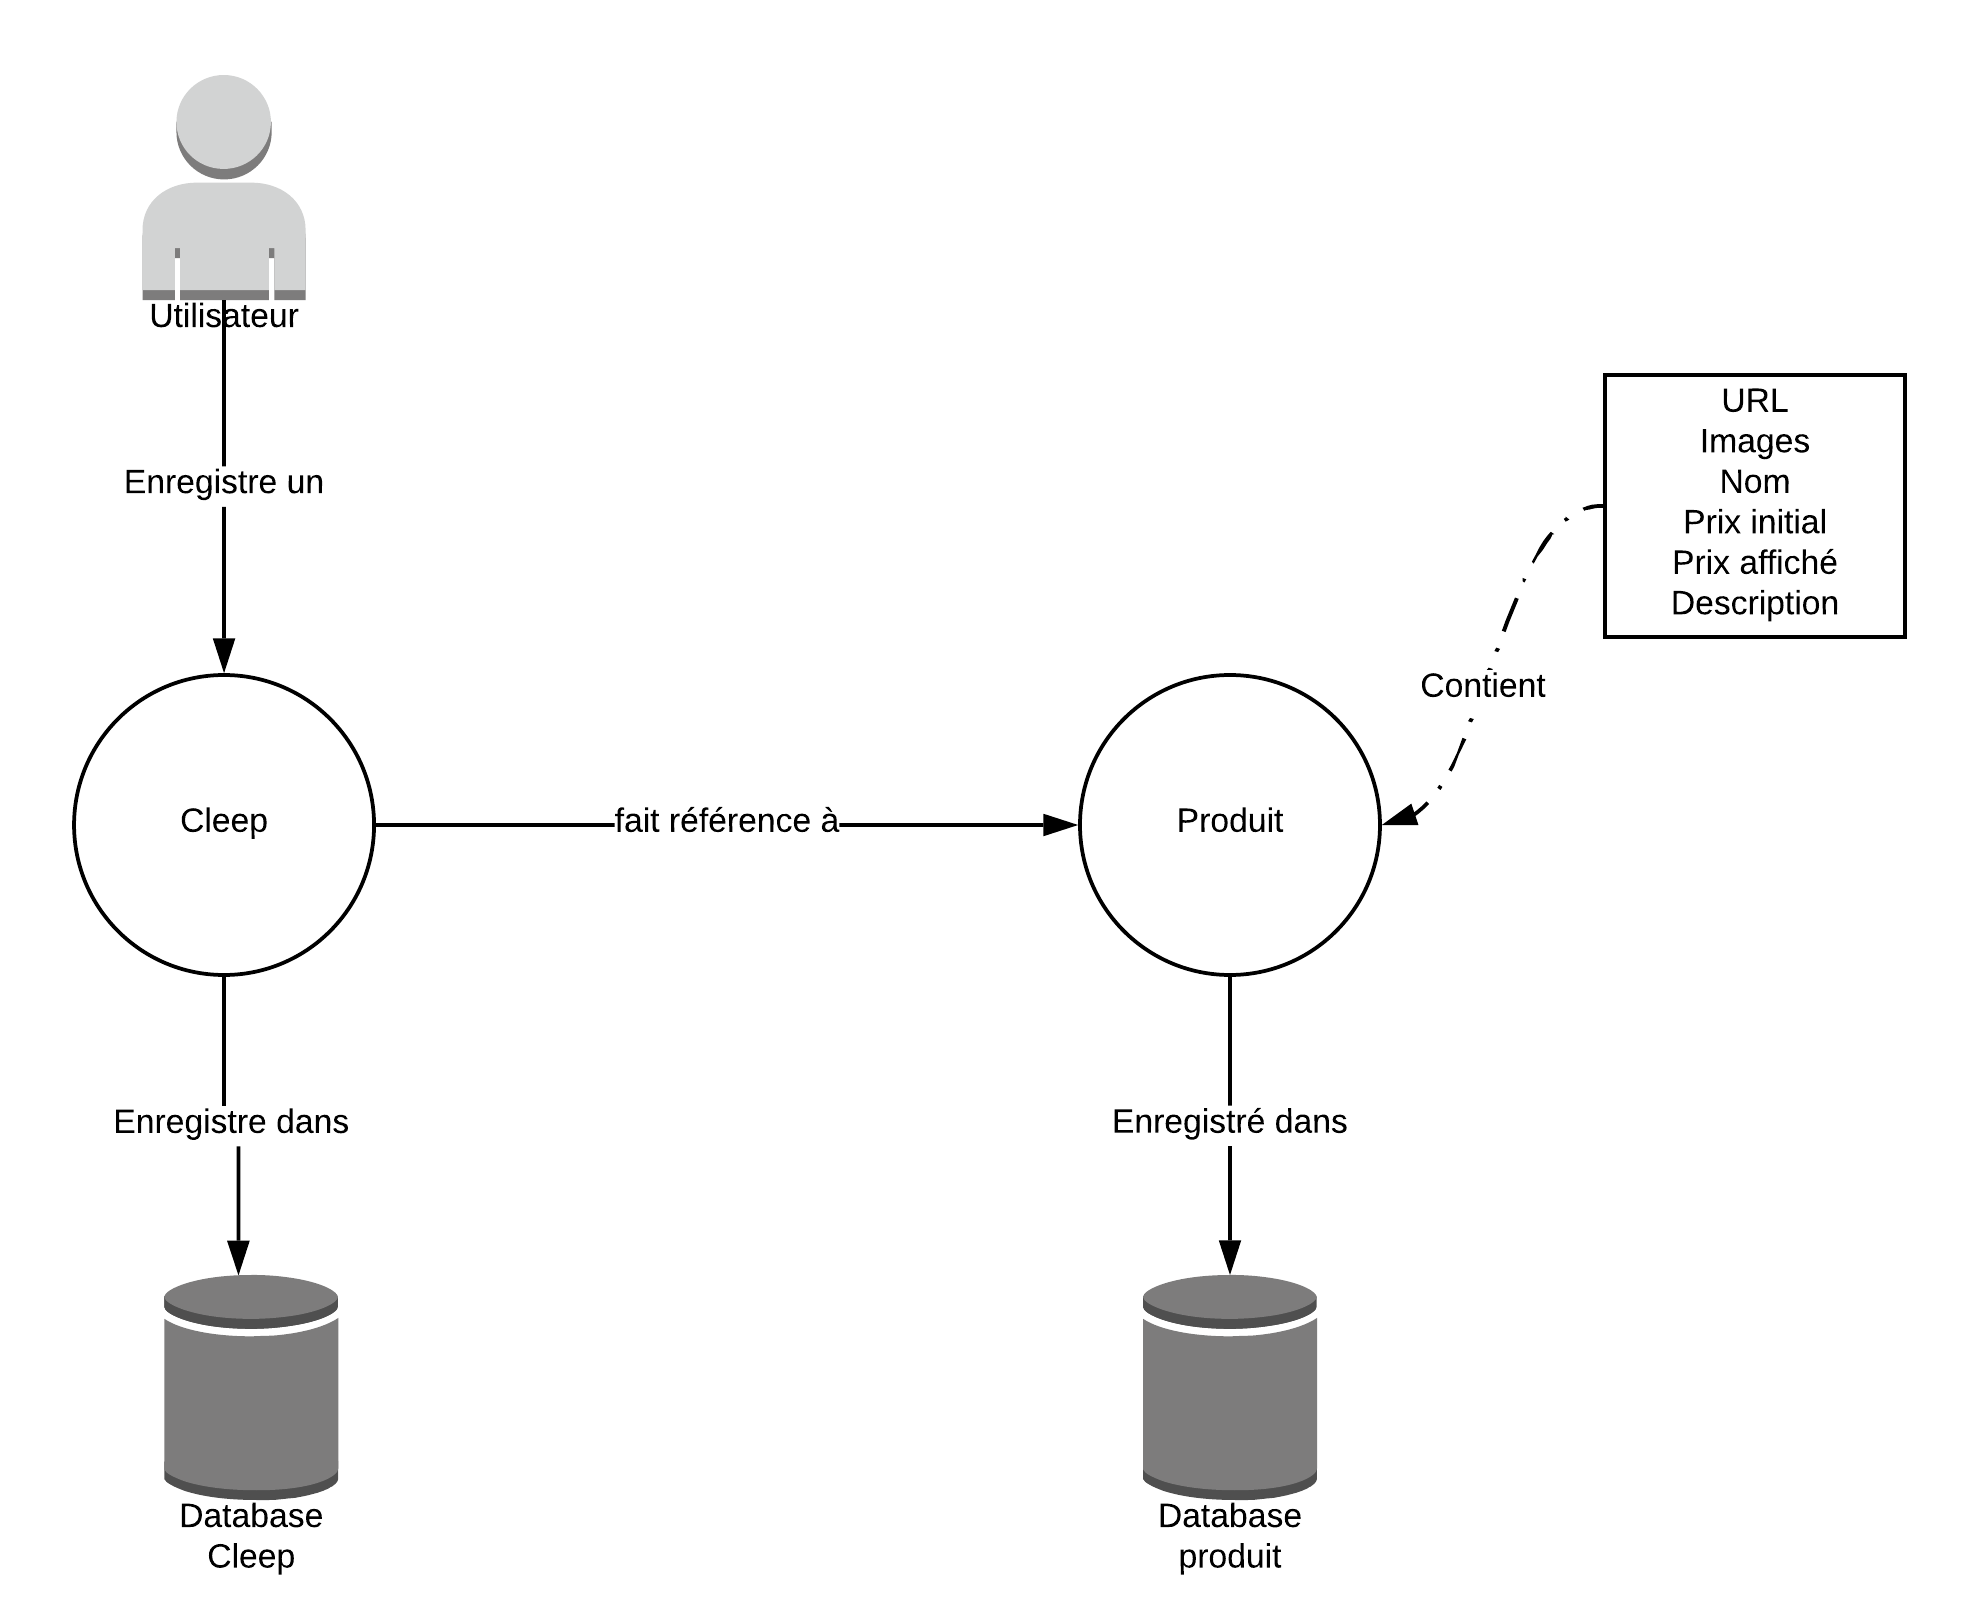
\includegraphics[keepaspectratio = true,scale=0.7]{scrapping.png}
	\caption{Organisation des données de cleep}
\end{figure}
\newpage

Relier un cleep à un produit est un défi pour l'application, car les utilisateurs sont plus enclins à rester dans l'environnement Cleep lorsqu'ils ont les informations à leur disposition dans l'application. En effet les cleeps contenant ces information, l'utilisateur est moins tenté de suivre le lien du produit et a plus de chance de rester sur l'application et parcourir les listes de clepp d'autres utilisateurs. \\
Cependant pour pouvoir faire cela, il faut récupérer les informations des produits au préalables. C'est ici qu'intervient le webscrapping. Les méta-données qui nous intéresse sont récupérées par ce moyen et entré dans la base de donnée. L'objectif de cette mission était donc d'enrichir la base de donnée des produits de manière automatique. 


\subsection{Travail effectué}
Cette sous-section relate le travail effectué sur cette mission.
\subsubsection{Contexte\\}
Avant mon arrivé, plusieurs methode de webscrapping étaient déjà utilisées:
\begin{itemize}
	\itemsep 0em
	\item Méthode automatique
	\item Méthode spécifique
\end{itemize}
\paragraph{Méthode automatique:\\}
Cette méthode était la plus utilisée pour récupérer les informations des produits. L'utilisateur rentre un lien dans l'application, par la suite ce lien est envoyé au serveur sur lequel la méthode est implémentée. Le serveur génère un navigateur internet sans interface graphique (headless browser) et requête le lien internet rentré par l'utilisateur. Ensuite, en analysant les balises du code HTML chargé, l'algorithme par certaines règles essaie de récupérer les méta-données. Ces informations sont alors transférés à l'utilisateur. Le schéma ci-après décrit le processus.
\begin{figure}[!h]
	\centering
	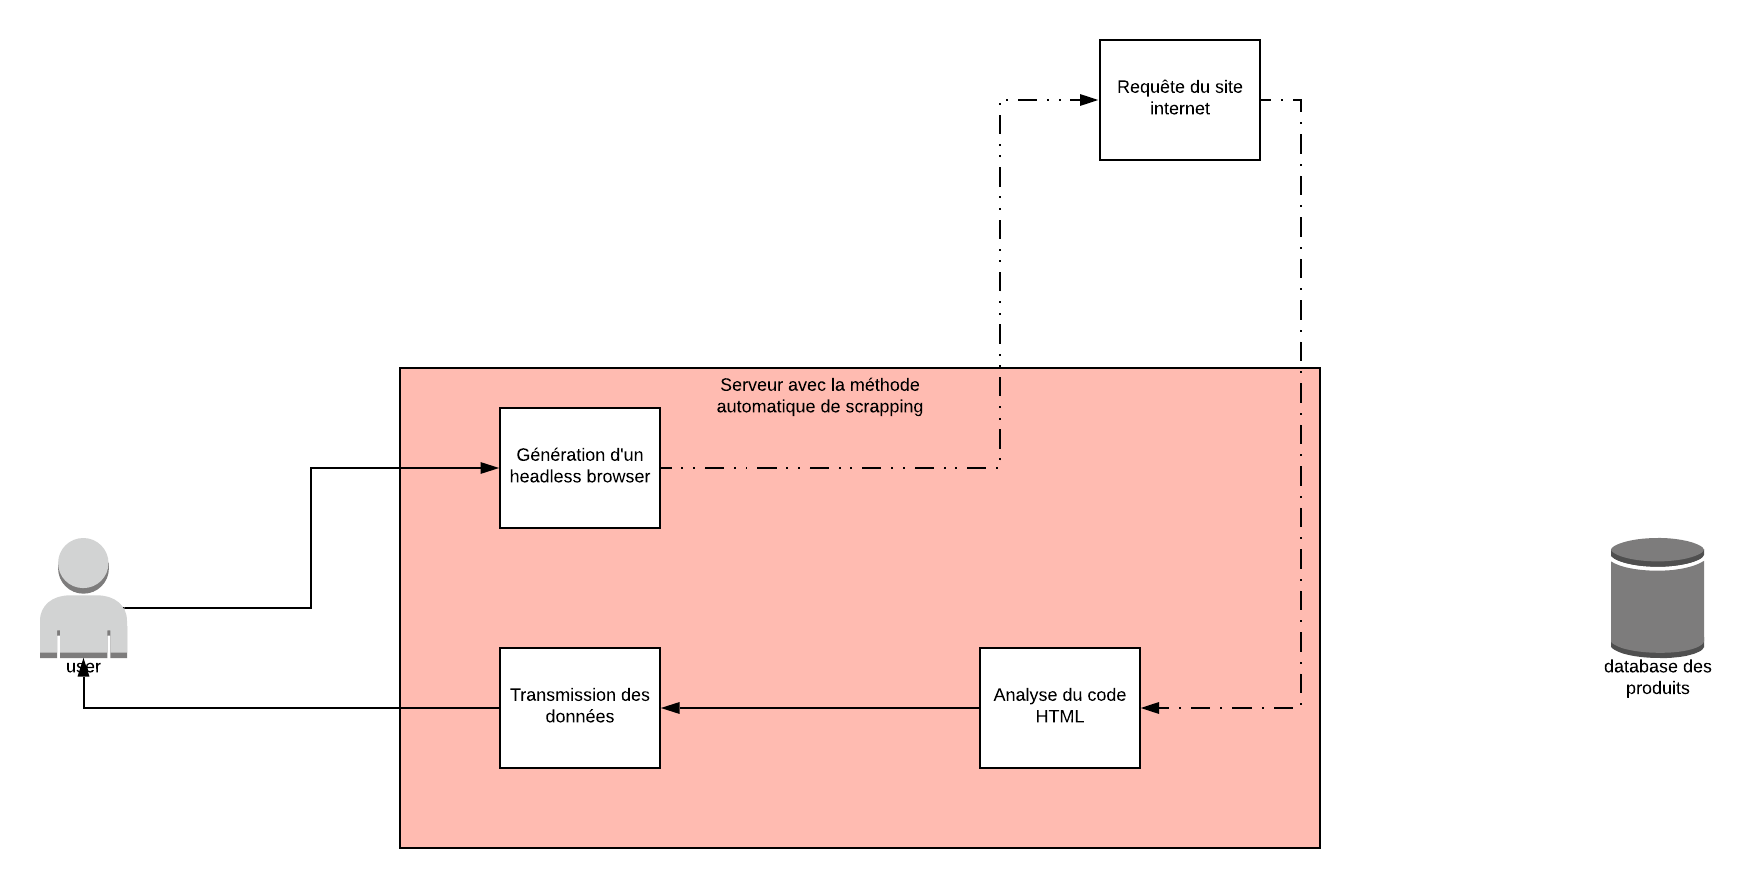
\includegraphics[keepaspectratio = true,scale=0.6]{browserInject.png}
	\caption{Méthode automatique}
\end{figure}
Bien que cette méthode de scrapping soit indépendant du site internet, elle reste néanmoins assez "précaire", car il est rare d'avoir toutes les informations nécessaires à disposition. Il est fréquent d'avoir certains attributs manquant, car les règles créées pour l'analyse du code HTML n'était pas assez vaste. Prenons les deux sites internet suivant :\\
\newpage
Site N°1:
\lstinputlisting[language=html]{site.html}

Site N°2:
\lstinputlisting[language=html]{site2.html}

Dans le cas N°1, il est facile de mettre une règle pour récupérer le prix dans le meta tag. Dans le cas N°2 cependant, le prix est "juste" inclut dans une balise <p>, rendant la règle précédente inutile. La méthode automatique implique donc beaucoup d'erreurs et d'approximations. Pour des soucis de mémoire, ces données ne sont pas enregistrées dans la base de donnée des produits, afin de ne pas garder les "fausse" données récupérées.
Cette méthode pose un autre soucis, c'est son temps de réponse. En effet, afin de scrapper le site, le serveur est obligé de générer un headless browser, de faire la requête, analyser le code HTML pour finalement retourner la réponse. Le temps de réponse doit être relativement bas, car l'utilisateur au moment du cleep doit pouvoir continuer ses activités sur Internet sans être interrompu trop longtemps par le temps que met Cleep à cleeper son produit, et donc eviter toute frustration.

\paragraph{Méthode spcéifique:\\}
C'est sur ce sujet que s'est concentré mon travail. Le principe de cette méthode est de prendre les sites internet un à un et d'appliquer un script de webscrapping qui leur est propre. Cela permet d'éviter les problèmes rencontrés précédemment.
La structure du code HTML derrière les pages produits est dans la quasi-totalité des cas la même pour un nom de domaine particulier. Il est possible que selon les sous-domaines d'un site cette page varie, par exemple pour la fnac on a:
\begin{itemize}
	\itemsep 0em
	\item https://livre.fnac.com/a13195869/Agnes-Martin-Lugand-A-la-lumiere-du-petit-matin
	\item https://jeux-video.fnac.com/a13608859/LEGEND-OF-ZELDA-LINKS-AWAKENING-FR-SWITCH-Jeu-Nintendo-Switch
	\item ...
\end{itemize}
Dans ce cas, on distingue les différents cas et ensuite on analyse le code HTML de chacune de ces pages. Cette méthode est bien plus fiable et donne de meilleurs résultats sur les méta-données requise.\\
Par ailleurs, afin de réduire le temps de réponse, une difficulté est rajouté : la génération d'un headless browser est supprimée m'obligeant à travailler avec le code source de la page (ie le résultat d'une requête cURL à la page), et les requêtes API.\\
En effet la génération d'un navigateur permettait de faciliter la tâche, car le code HTML étant totalement généré, il suffisait de récupérer le contenu des balises afin d'obtenir les informations nécessaires. Cependant via une requête cURL (ie le code source de la page), les script JavaScript ne sont pas déclenchés, il faut donc chercher au travers des differents script et requêtes API les éléments que l'on souhaite récupérer.

\begin{figure}[!h]
	\centering
	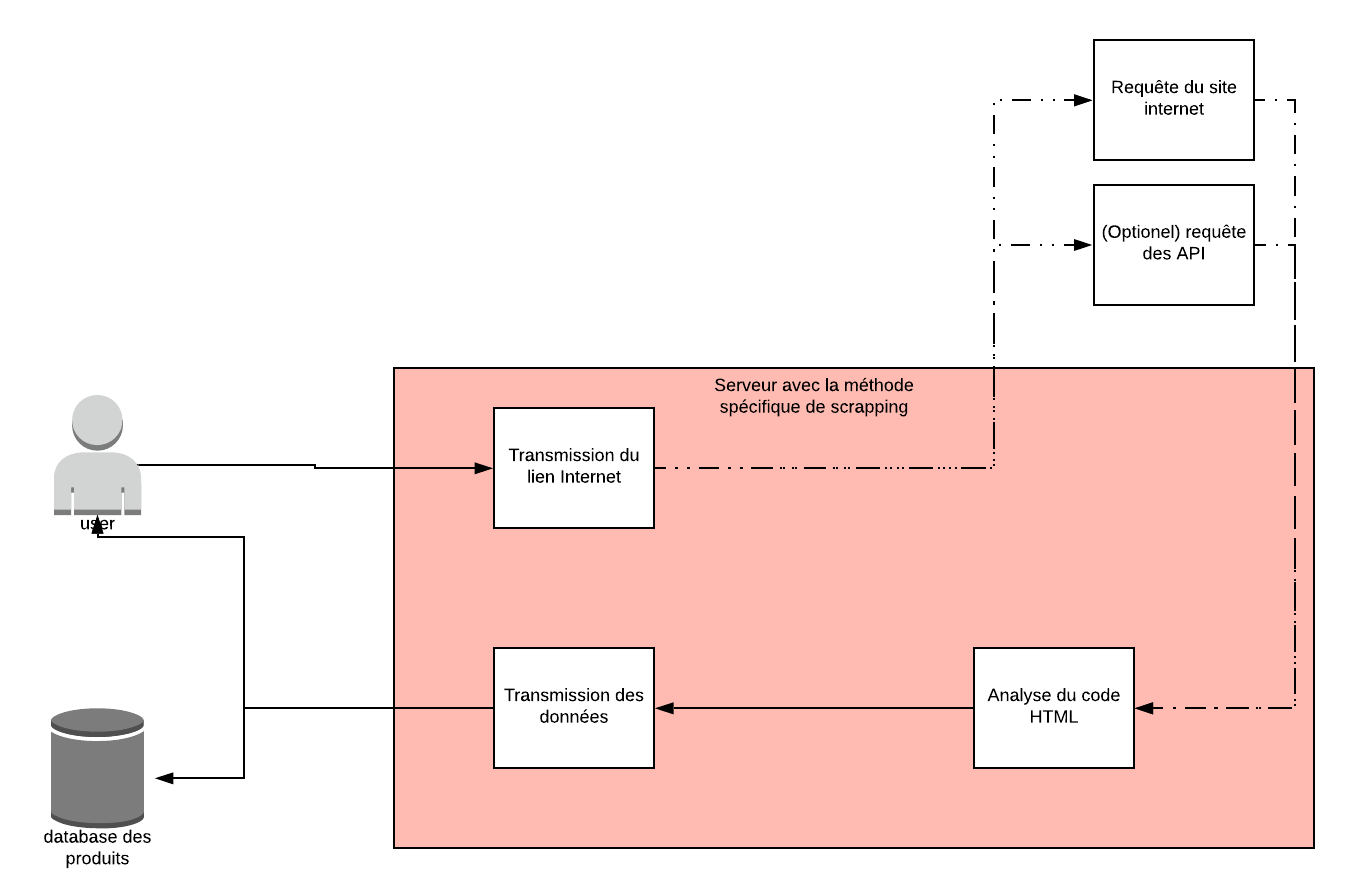
\includegraphics[keepaspectratio = true,scale=0.6]{specific.png}
	\caption{Méthode spécifique}
	\label{fig:methspec}
\end{figure}

\newpage

\paragraph{Démarche\\}
Le processus \textbf{figure \ref{fig:methspec}} montre les différentes étapes de la méthode spécifique. Mon travail s'est principalement concentré sur l'algorithme analysant un site web en particulier et la gestion des requêtes.\\
Prenons l'exemple suivant \cite{fnac} :
\begin{figure}[!h]
	\centering
	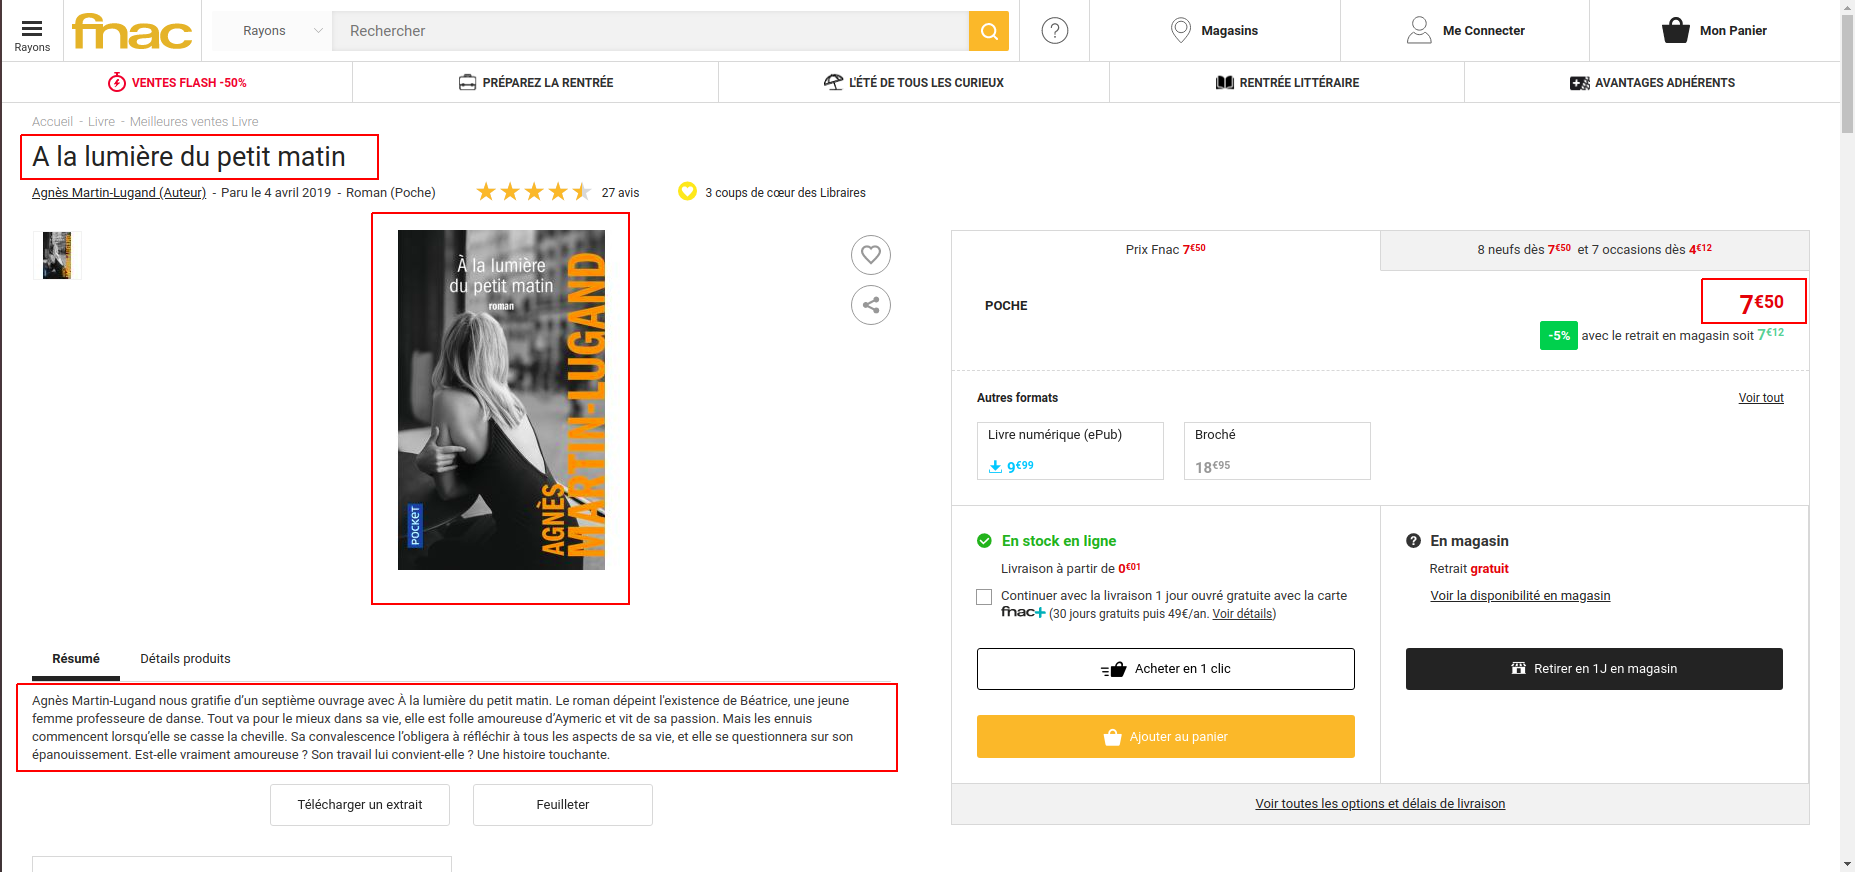
\includegraphics[keepaspectratio = true,scale=0.25]{fnac.png}
	\caption{Exemple fnac}
\end{figure}
Les encadrés rouges correspondent aux éléments que l'on doit récupérer. Vous pouvez retrouver en annexe une version allégé du code HTML (Annexe 9.1). Il est alors facile de comprendre que récupérer l'attribut $data-src-zoom$ de la balise <li> nous permet de récupérer l'image et le JSON quant à lui permet de récupérer les autres éléments requis.\\
La démarche adopter pour scrapper les différents sites à toujours été la même. Tout d'abord on analyse le code source afin de savoir quels éléments sont à récupérer. Ensuite on teste avec plusieurs liens différents afin de tester la robustesse de l'algorithme. Une validation finale était faite côté client, et ensuite l'algorithme était mis en production.\\ \\
Le dernier point nécessitant du travail : où trouver les liens permettant de scrapper les produits et peupler la base de donnée? L'ensemble des liens déjà cleepés sont enregistrés, et donc peuvent être utilisé pour répondre à cette question. Le client possédait déjà un script permettant de trier les liens par nom de domaines. Ainsi pour chaque nom de domaine que j'ai traité, j'ai du trié les liens pertinents (ie de produits) des liens inutiles (page principal, page de catégories etc). Par exemple, pour la fnac certains utilisateurs ont cleepé des pages présentant plusieurs produit \cite{mve} ce qui ne convient pas au processus détaillé auparavant.

\paragraph{Résultats\\}
A la fin de cette mission, j'ai développé un script de webscrapping pour plus de 56 sites différents. Cela a permis à Cleep de peupler sa base d'environ 220 000 produits différents.\\
Sur une vision plus large, les utilisateurs passent en moyenne plus de temps sur l'application (effet recherché), mais aussi ils ont tendance à cleeper plus de produit sur les sites dont le webscrapping a été fait.

\subsection{Vision critique et apport personnel}

La mission de webscrapping était plutôt simple, dans le sens qu'une fois les notions de webscrapping acquises, cette mission consistait à analyser un code HTML et les requêtes faits en javascript, pour trouver les informations nécessaires. Mon apport personnel s'est plus concentrés sur les discussions avec le client au sujet de l'amélioration du scrapper générique et le choix des technologies ainsi que la compréhension de l'infrastructure de Cleep.

\subsubsection{Scrapper générique\\}
Le scrapper générique déjà présent n'était pas assez efficaces pour pouvoir enregistrer les données des produits et il était trop lent pour être utilisé en production indéfiniment (pour l'instant, si un lien n'appartient pas à la liste des 56 domaines scrappés, il passe par le scrapper générique). Comme il n'est pas non plus possible de scrapper de manière spécifique l'ensemble des sites commerciaux existants (la base de donées de Cleep compte plus de 8000 nom de domaines différents), j'ai discuté avec le client sur la nécessité d'un scrapper générique plus performant.\\
Ainsi en parallèle, j'ai essayé de developper un scrapper générique plus performant n'utilisant pas un "headless browser". La valeur ajouté de Cleep reposant sur les images du produit enregistré dans l'application, j'ai travaillé sur un scrapper générique permettant de récupérer les images du produit.\\
Ce scrapper suit les 2 étapes suivantes :
\begin{itemize}
	\itemsep 0em
	\item Récupérations des liens "dynamique" de la page HTML
	\item Clustering des liens
\end{itemize}
\paragraph{Récupérations des liens "dynamique" de la page HTML:\\}
Cette étape consiste à récupérer l'ensemble des liens images de la page n'étant des liens statique. Un lien image est considéré comme statique s'il est présent plusieurs fois sur différentes pages. En générale ces images sont les logos et autre widgets communément présents. L'exemple \textbf{figure \ref{fig:stats}} ci-après montre les images statiques sur le site de la fnac. Une fois connus, ces liens ne sont pas pris en compte par le scrapper générique.\\ 
Ainsi, à la fin de l'étape 1 (cf \textbf{figure \ref{fig:step1}} pour voir le procédé), l'ensemble des liens dynamique (ie liens d'images changeantes) est connu. Cependant, parmis ces images nous avons les images du produits, mais aussi celle fournies par les recommandations. Il faut donc trouver un moyen de séparer ces images .

\begin{figure}[!h]
	\centering
	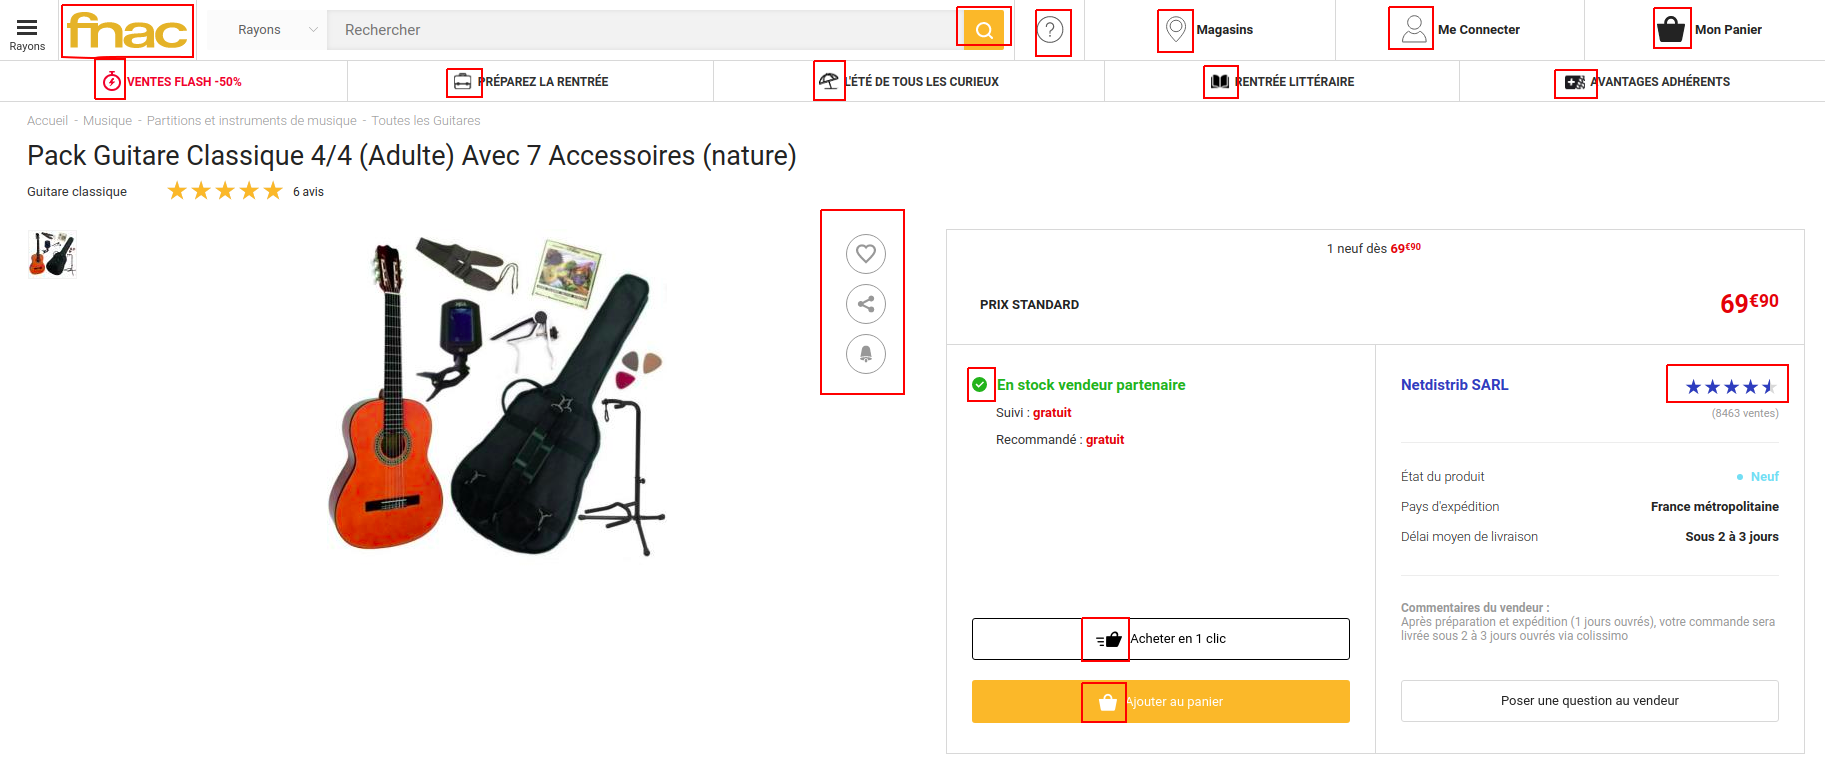
\includegraphics[keepaspectratio = true,scale=0.25]{static.png}
	\caption{Exemple d'images statiques}
	\label{fig:stats}
\end{figure}

 
\begin{figure}[!h]
	\centering
	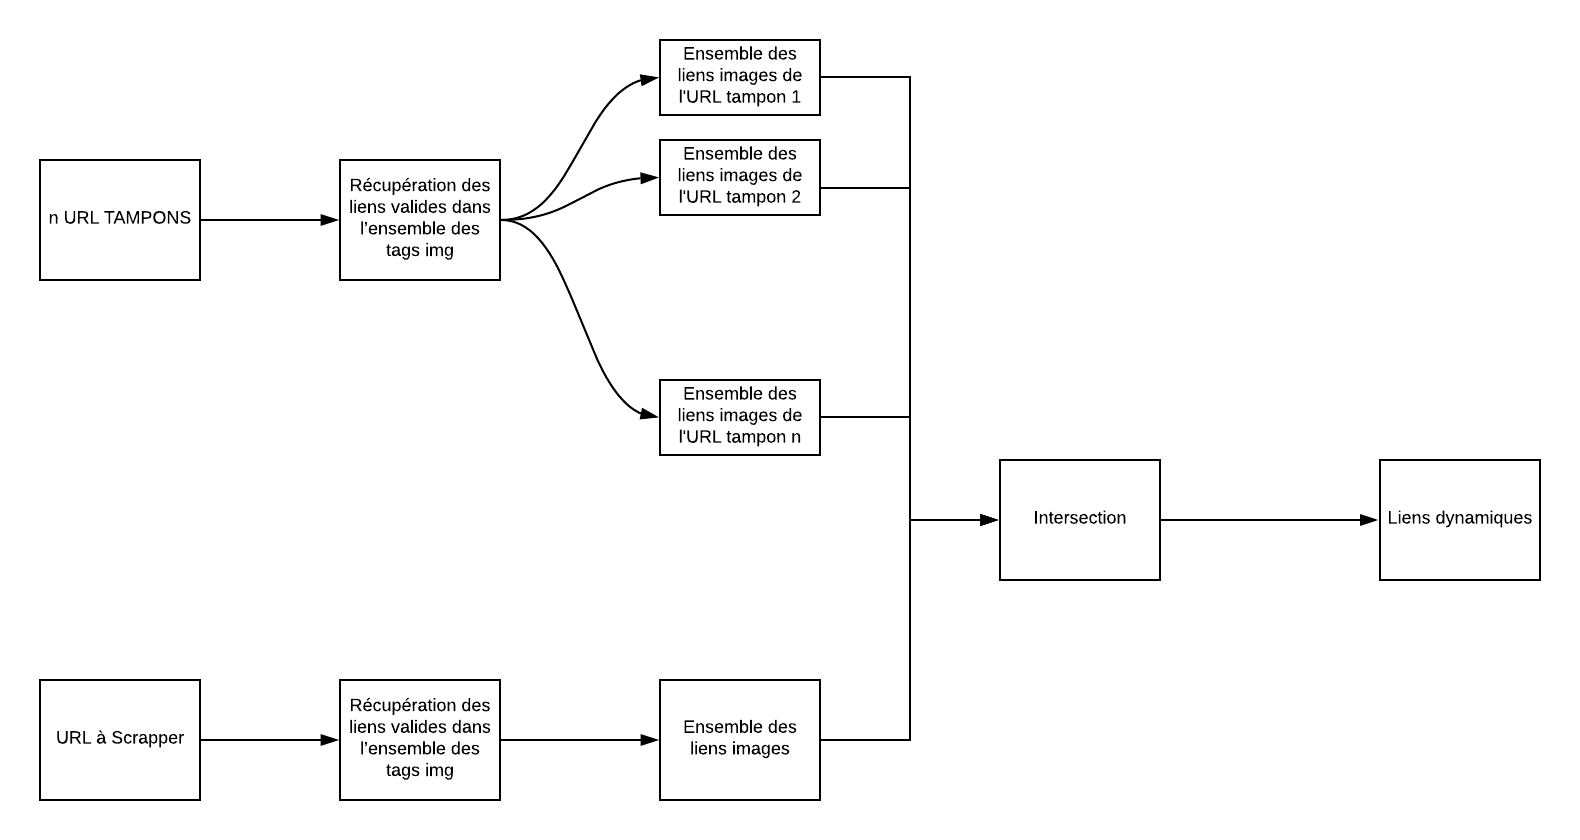
\includegraphics[keepaspectratio = true,scale=0.4]{step1.png}
	\caption{Etape 1}
	\label{fig:step1}
\end{figure}

\paragraph{Clustering des liens\\}
Le but ici est de regrouper les liens de recommandations entre eux et les liens concernant le produits entre eux aussi. Pour cela j'ai utilisé un algorithme de clustering : dbscan. Le clustering se fait sur la distance en nombre de caractère dans le code HTML par rapport au début du code.\\
Cela permet donc d'avoir en général 2 cluster distincts. En me basant sur l'ensemble des sites que j'ai scrappé auparavant, le 1er cluster est choisi comme celui contenant les images que l'on souhaite. Ainsi à la fin de cette étape on est sensé avoir l'ensemble des images du produit. Afin de vérifier si les liens sont bien ceux recherchés, on compare les liens entre eux en utilisant la distance de Levenshtein \cite{levenshtein}. La distance de Levenshtein entre deux chaînes de caractère $A$ et $B$ est le nombre minimum de transformation (ajout/suppression/changement d'un caractère) pour passer de $A$ à $B$. Ainsi, si dans le cluster, un lien paraît plus éloigné des autres, il est retiré de la liste.\\
Cette règle se base sur le fait que les images d'un même produits ont souvent des liens très similaires et sont différencié par un identifiant dans l'URL. 

\paragraph{Tests et résultats\\}
Les tests ont été réalisé sur une vingtaine de site que j'avais au préalable scrapper afin de pouvoir évaluer la différence. Il apparaît que ce scrapper générique arrive à récupérer toutes les images d'un produit spécifique. Cependant, il récupère trop d'image dans le sens où il peut récupérer 4 fois la même image mais ayant des tailles différentes. Encore une fois, pour des raisons de capacités mémoire, cette solution n'a pas été retenue par le client en l'état, mais est toujours en cours de développement.


\subsubsection{Technologie utilisée\\}
L'ensemble du travail a été réalisé en NodeJS (interpreteur Javascript). Cette technologie a été utilisé car l'ensemble de l'architecture client était en NodeJS. Il était possible de travailler avec les librairies Python permettant de scrapper et faire des requetes HTML (scrappy, beautifulsoup) car cette partie est plutôt indépendante. Cependant pour éviter l'overhead introduit par un changement de langage, j'ai préféré suivre le langage du client.\\
Par ailleurs, plusieurs sites internet ont des protections vis à vis du webscrapping. En effet les requêtes fait aux différents serveurs affecte les capacités de ces derniers. Ainsi deux problèmes se sont posés:
\begin{itemize}
	\itemsep 0em
	\item Ne pas lancer "involontairement" une attaque contre les serveur du site en question: pour cela on a trouvé une certaine limite temporelle avec le client
	\item Les adresses IP des serveurs de Cleep qui étaient déjà sur liste noire de plusieurs sites.
\end{itemize}

Le deuxième problème s'explique par une technologie de protection employé par les site internet contre le webscrapping : Datadome. Datadome detecte si une requête est faite par un utilisateur ou un robot en regardant si le javascript de la page est chargé et executé. Si ce dernier n'est pas executé, il s'agit probablement d'un bot ayant requêté uniquement le code source de la page, ce qui est exactement notre cas. Une fois detecté par Datadome, l'adresse IP qui a servi pour la requête est mise sur liste noire et il n'est plus possible de faire de requête.\\

La solution trouvé avec le client est de passer par un service de Proxy payant : Luminati, qui permet de changer d'adresse IP à chaque requête et donc de pouvoir utiliser les scripts de scrapping. Il est a noté que ce service facture à la requête, ainsi seul les sites ayant une protections datadome ou similaire passent par ce proxy.

\newpage

\section{Mission : Moteur de recommandation pour Cleep (3 mois)}

Cette partie est consacrée au développement d'un moteur de recommandation pour la start-up Cleep. Cette mission fait directement suite à celle de webscrapping et reste dans l'esprit de développer des fonctions nécessaires à la croissance de l'application. Lors de cette mission, j'ai profité d'une grande autonomie car aucune solutions antérieures n'existaient auparavant. J'étais cependant en contact avec Damien Meurisse, co-fondateur de Cleep, et Paul Saffers, consultant datascientist à Sia Partners, afin de critiquer et valider mon avancement 

\subsection{Contexte et problématique}

Le but de cette mission est de développer un moteur de recommandation : à partir d'un élément et des données qui lui sont liées, le moteur doit retourner un ou plusieurs éléments similaires. Cette pratique est vastement répandue parmi les sites marchands/ sites de services (Amazon, Netflix, Pinterest ...).\\

Avant le début de cette mission, Cleep n'avait pas de moteur de recommandation à proprement dit, certaines ébauches de moteur avait été faites, mais rien de concret. Pour une application comme Cleep dont le principe est de rendre l'utilisateur indépendant des sites marchands et de lui offrir une alternative au shopping basique sur Internet, la création d'un moteur de recommandation devenait nécessaire.\\
En effet, il est possible de partager au travers de l'application les produits cleepés ainsi que les listes de cleeps. Un utilisateur peut donc voir les cleeps d'autres utilisateurs et en particulier ceux correspondants à ses centres d'intérêts. Les interactions avec les cleeps déjà disponibles sur la plateforme sont donc importantes, plus un utilisateur navigue sur Cleep, plus il passe de temps sur l'application ce qui le fidélise. Cependant sans moteur de recommandation, la navigation et la découverte de nouveaux cleeps est assez difficile pour l'utilisateur. Celle-ci passe soit par la bar de recherche pour la recherche de cleep(s) spécifique(s), soit par les pages catégories (triant les cleeps des utilisateurs par catégorie).\\
C'est donc dans l'optique de créer un moteur de recommandation fonctionnel et adapté à l'architecture déjà présente de Cleep que la mission m'a été confiée.

\paragraph{Objectif(s)\\}

L'objectif premier de cette mission qui a durée 2.5 mois était de créer un moteur de recommandation à partir des données de Cleep. Cette mission s'est divisée en deux grandes étapes:
\begin{itemize}
	\itemsep 0em
	\item Etudes des différents moteur de recommandations existant et études des bases de données en graphe
	\item Implémentation sur la technologie choisie d'un moteur de recommandation pour Cleep
\end{itemize}
La deuxième étape inclue l'ensemble des discussions avec le client au sujet des caractéristiques du moteur de recommandation, comment il est sensé se comporter, les améliorations possibles par rapport au cas de Cleep, ainsi que les manières de tester et valider la solution apportée.\\
Dans le cas précis de Cleep, un moteur de recommandation consiste à fournir à partir d'un cleep un certains nombre de cleep pouvant être utile à l'utilisateur (cf schéma \textbf{figure \ref{fig:reco}}). 

\begin{figure}[!h]
	\centering
	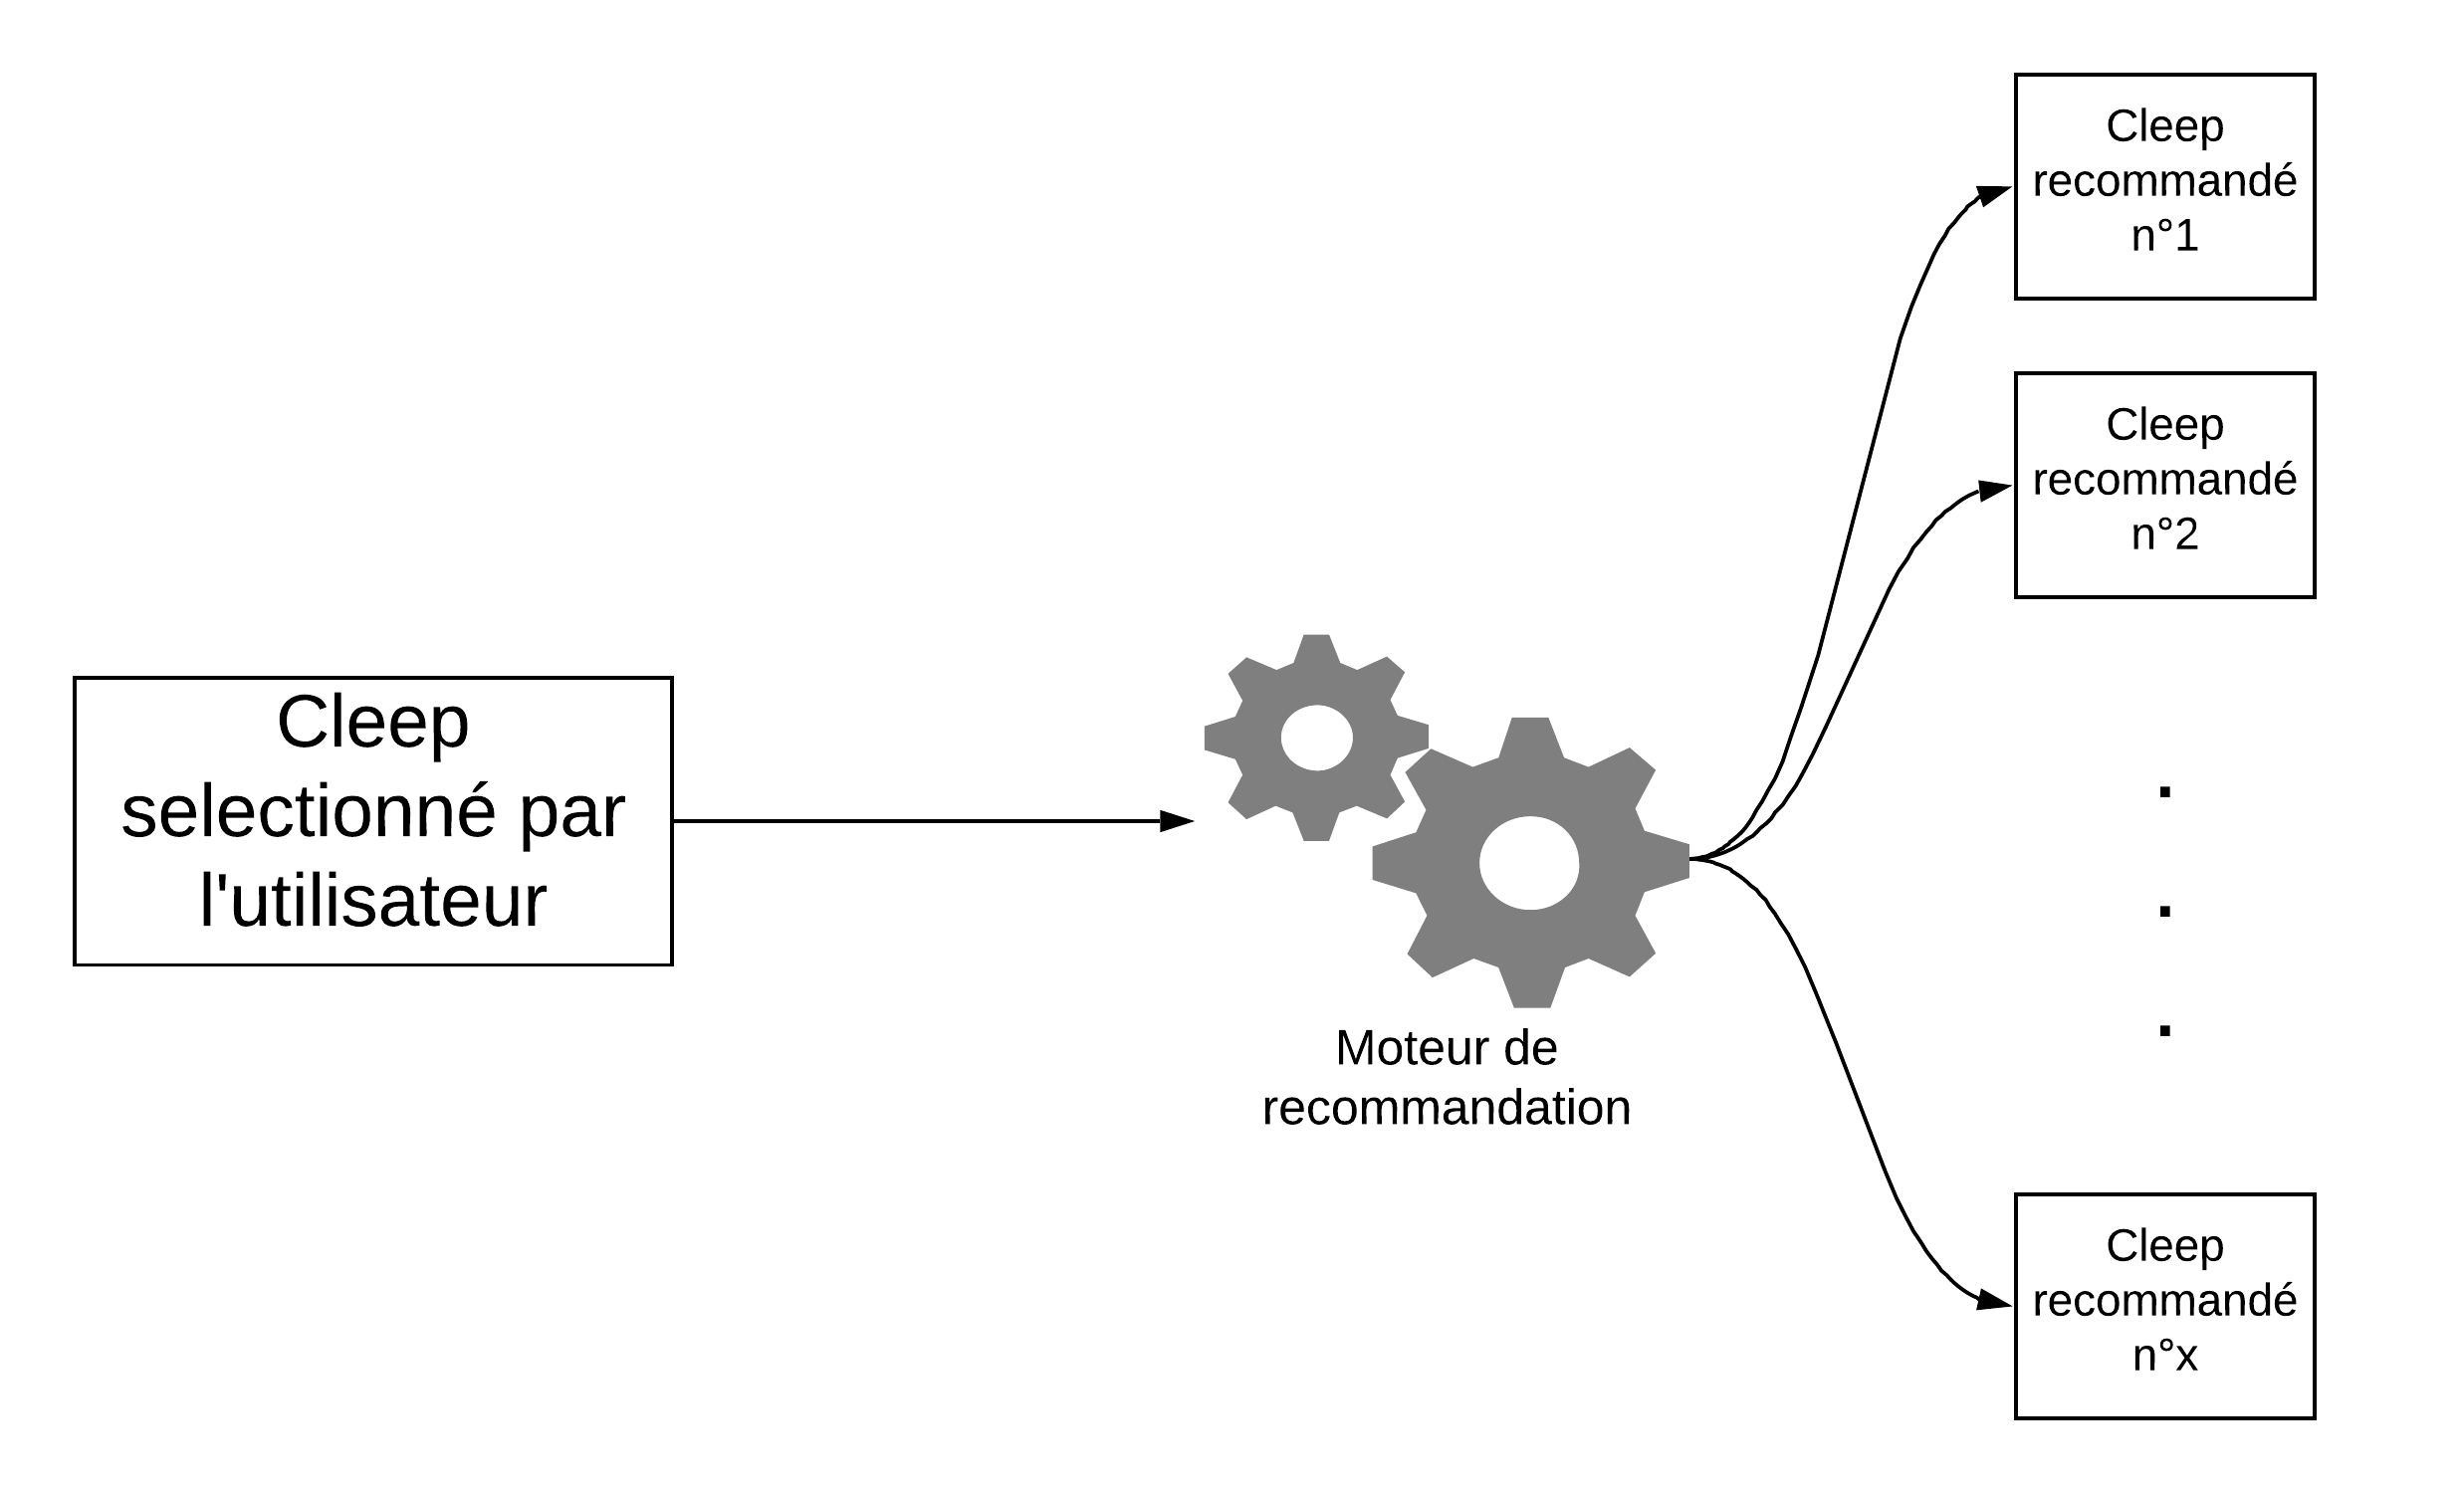
\includegraphics[keepaspectratio = true,scale=0.4]{reco.png}
	\caption{Etape 1}
	\label{fig:reco}
\end{figure}

La boite noire qu'est pour l'instant le moteur de recommandation reposera sur l'ensemble des éléments présents dans la base de donnée de Cleep afin d'avoir des recommandations précises et pertinentes. En effet, plus l'analyse des données et de leurs relations est poussée, plus le moteur retournera des cleeps pertinents. Tout du moins pertinent par rapport aux tendances évoquées par les données.

\paragraph{État initial}
Avant le début de ma mission, il y avait déjà eu quelques idée pour la création et le développement d'un moteur de recommandation.\\
Cleep est une application qui repose beaucoup sur le visuel, et donc sur les images des produits. Cette image permet à l'utilisateur de reconnaître la nature du produit et donc de savoir ce qu'il a cleepé. Ainsi une idée envisagée était de baser le moteur de recommandation uniquement sur l'analyse des images. Pour cela il existe une API developpé par Google qui permet de fournir des "tags images" ainsi qu'une pourcentage de confiance associé. Dans la \textbf{figure \ref{fig:ggviz}}, on peut voir l'application de l'algorithme derrière cette API sur un pull.\\

\begin{figure}[!h]
	\centering
	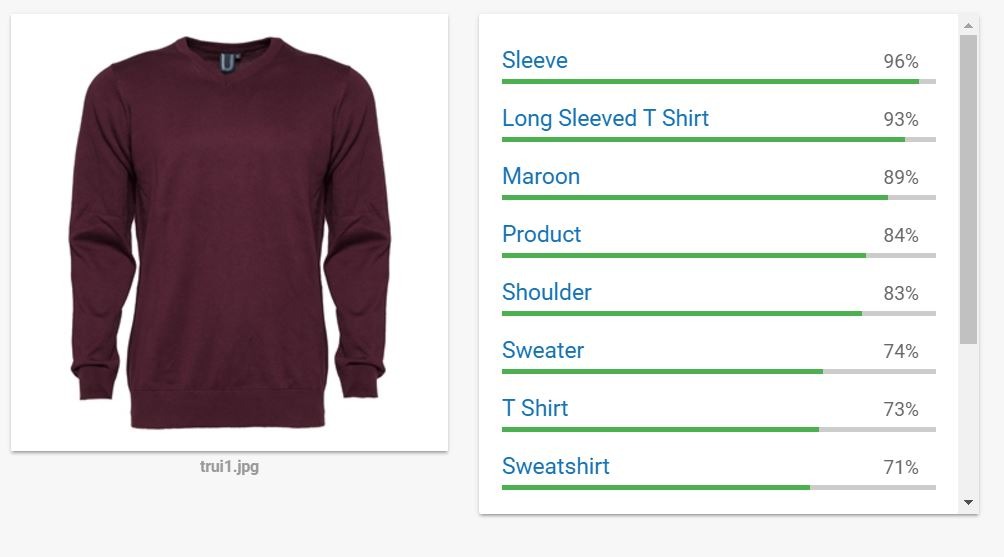
\includegraphics[keepaspectratio = true,scale=0.4]{ggvision.jpg}
	\caption{Etape 1}
	\label{fig:ggviz}
\end{figure}

Dans cette ébauche de moteur de recommandation, l'idée était donc de tagger toutes les images de la base de donnée en premier lieu. Ensuite, pour un cleep dont on veut les recommandations, on fait passer ses images par le même algorithme, et on récupère ses tags. La dernière étape du processus envisagé est de retourner les images ayant le plus de tags en commun avec ceux du cleep original, tout en prenant en compte le pourcentage de confiance.\\
Cette idée, bien que fonctionnelle, ne prend en compte qu'une infime partie de la base de donnée de Cleep (ie les images). Ainsi, il est très peu personnalisé et retourne des recommandations génériques. Le but premier de cette mission est donc d'utiliser au mieux l'ensemble des informations afin de fournir des recommandations personnalisées.

\paragraph{Écosystème de Cleep\\}
Il est nécessaire pour comprendre le travail que j'ai effectué de connaître l'ensemble des éléments à disposition dans la base de donnée Cleep. Je reviendrais plus en profondeur par la suite, en détaillant précisément le type de base ainsi que la structure choisie pour faire fonctionner ce moteur de recommandation.\\
\newpage

La base de donnée est composé de:
\begin{itemize}
	\item Informations de l'utilisateur anonymisées : son âge, son sexe, ses interêts ses interactions avec les sites internet marchands etc.
	\item Informations sur les cleeps : la liste à laquelle il est associé, ses tags provenant de google vision, sa date de créations, l'utilisateur qui l'a créé, et son statut (s'il est toujours en ligne ou s'il a été supprimé par son propriétaire)
	\item Information sur les listes de cleeps: son statut, son propriétaire et l'ensemble des personnes ayant accédé/partagé cette liste
\end{itemize}
Par ailleurs, les activités des utilisateurs sont enregistrées, ce qui donne des informations en plus, notamment sur les interactions entre les trois entités : cleeps, utilisateurs, listes. Sont a disposition les activités sur les relations suivantes:
\begin{figure}[!h]
	\centering
	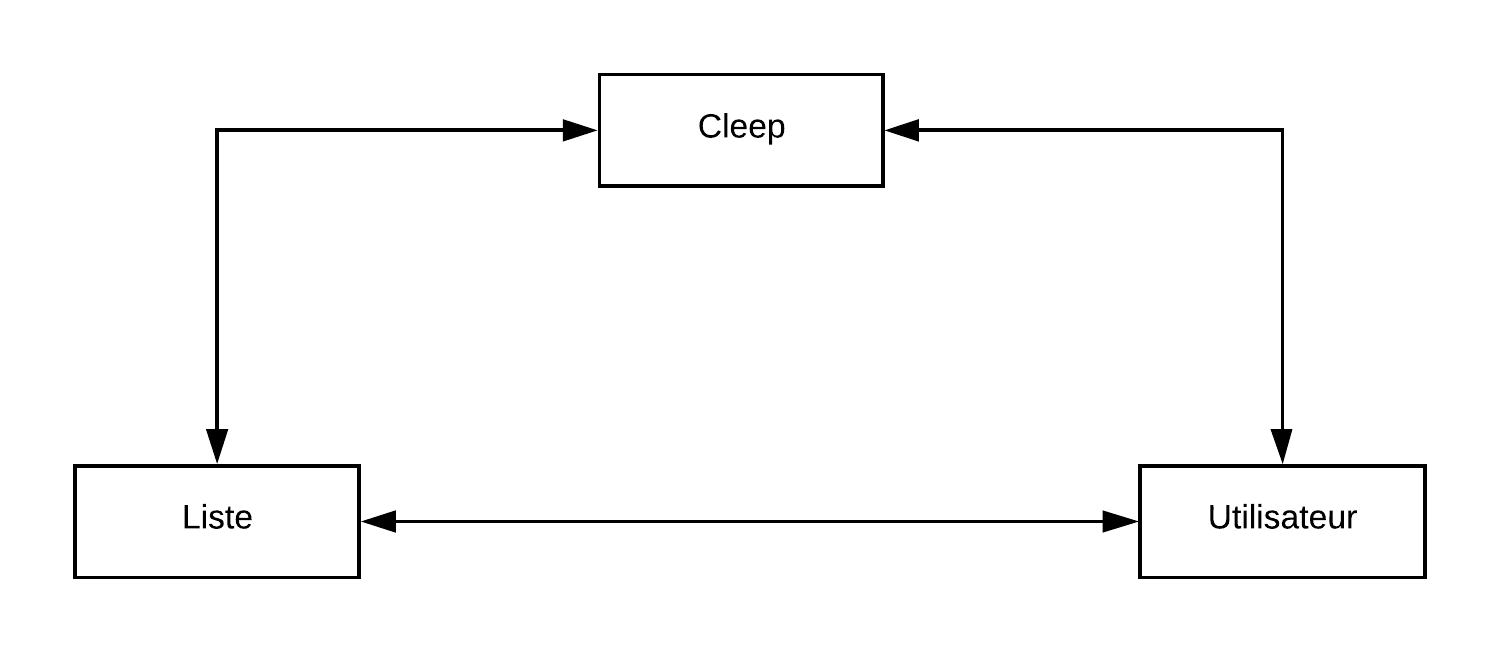
\includegraphics[keepaspectratio = true,scale=1]{relations.png}
	\caption{Etape 1}
	\label{fig:rel}
\end{figure}



\subsection{Travail effectué}
Dans cette partie je vais décrire le travail effecuté pour la création du moteur de recommandation et revenir sur les principales étapes de ce processus. Comme dit précédemment, cette mission s'est d'abord axée sur l'étude des système de recommandations déjà existant ainsi que les technologies qui leurs sont associées. Ensuite, il a fallu designer et implémenter le moteur de recommandation en se basant sur les conclusions de la première partie. 

\subsubsection{Étude des moteur de recommandations similaires}

Le cas de Cleep n'est pas du tout unique, il y a plusieurs exemples d'application similaires sur le marchés utilisant des moteurs de recommandations. On peut penser notamment à l'ensemble des sites marchands que j'ai scrappés en première partie. Chacun d'entre eux possède un système leur permettant de recommander des produits à partir d'un article.\\
Il y a donc autant de manière de faire un système de recommandation qu'il y a de site en proposant. Cependant il y a des objectifs clairs vis à vis de ce dernier :
\begin{itemize}
	\itemsep 0em
	\item A partir d'un articles, plusieurs articles doivent en ressortir
	\item La recommandations doit être personnalisée
	\item La recommandation doit être rapide
	\item La mise en place du système ne doit pas être chère
\end{itemize}
C'est donc avec ces objectifs que j'ai commencé les recherches.

\subsubsection{Article de recherche : moteur de recommandation de Pinterest\\}
Après quelques recherches, ma culture personnelle  ainsi que sur les conseils de Damien et Paul j'ai orienté mes recherches sur les moteurs de recommandations ayant une solution basé sur le parcours de graphe. Damien m'a alors recommandé la lecture de l'article de recherche sur le moteur de recommandation de Pinterest : Pixie \cite{pixie}.\\
Pinterest \cite{Pinterest}, est un réseau social, dont le principe est de partager de l'information via des photos, vidéos, GIFs. Chaque élément partagé peut avoir une description un titre et des tags au choix de l'utilisateur. Ce réseau est en général utilisé pour partager autour de certains centres d'intérêts comme par exemple la photographie, le sport, la cuisine etc. Le moteur de recommandation de Pinterest est donc une bonne source d'inspiration pour Cleep. Le parallèle se faisant sur le côté très graphique de l'application. Ce sont les images qui attirent l'œil avant tout, mais aussi sur le but du moteur qui est d'identifier les pins (entité regroupant l'ensemble des informations liés aux images sur Pinterest)/cleeps répondant au mieux à l'envie de l'utilisateur. Ainsi, pour les deux application ce n'est pas nécessairement de pousser à l'achat, mais de faire rester sur l'application qui est important.\\

Pixie est un moteur de recommandation basé sur le parcours d'un graphe en marche aléatoire. Le graphe créé pour Pixie se base sur l'ensemble des entités présentes dans l'écosystème Pinterest. Pour résumer, les noeuds du graphe sont les pins et les utilisateurs. Les arrêtes sont les relations : pins $\leftrightarrow$ pins, pins $\leftrightarrow$ utilisateurs, utilisateurs $\leftrightarrow$ pins. Chacune des entités (arrêtes et nœuds) contiennent de l'information.\\
Le graphe établit, il est alors possible d'établir une distance entre les pins. Cette distance est très importante car c'est elle qui va déterminer la qualité du moteur de recommandation. Le calcul de cette distance est spécifique à Pinterest, je ne vais donc pas la décrire. Cependant il est à noter que Pinterest utilise la quasi-totalité de l'information qu'il possède afin de calculer cette distance.\\
Il est possible de penser que le travail est fait et qu'il suffit uniquement de récupérer pour un pin les pins les plus proche de ce dernier sur le graphe. Cependant, comme le titre du papier de recherche l'indique, il y a plus de 3 milliards de pins et plus de 200 millions d'utilisateurs. Ainsi, pour chaque nœud il faudrait calculer la distance avec l'ensemble des autres nœuds, ce qui est très long voir impossible. Mais aussi il faudrait stocker cette donnée ce qui est aussi compliqué vu la taille des données. En effet, en supposant que le résultat soit un entier codé sur un 4 octets mais aussi que la distance pour aller d'un pin A à un pin B soit indépendant du chemin, il faudrait pour un nœud 12 gigaoctets. Soit pour l'ensemble de la base de donnée 36 exaoctets ($36.10^9$ $Go$). De plus, à chaque ajout de nœuds, il faudrait tout recalculer, car les relations peuvent changer.\\
Les problèmes de stockage, de calculs mais aussi de mise à jour en temps réel rendent la solution évoquée précédemment irréalisable. De plus vu que les arrêtes du graphe portent de l'information, la distance dépend bien du chemin parcouru ainsi les calculs ont été (volontairement) vu à la baisse.\\

Le papier répond à ces problèmes avec l'heuristique suivante (exemple \textbf{\ref{fig:procpint}}):
\begin{itemize}
	\itemsep 0em
	\item Étape 1 : Récolte des informations sur le premier Pin
	\item Étape 2 : N marches aléatoires sur le graphe ($N \in \mathbb{N}$ )
	\item Étape 3 : Calcul du score (distance) pour chaque marche aléatoire avec le dernier pin disponible sur la marche.
	\item Étape 4 : Parmis les N scores, seul les pins recommandés ayant un socre supérieur à un seuil déterminé au préalable sont gardés
	\item Étape 5 : S'il n'y a pas assez de pins pour la recommandation, le processus est relancé 
	\item Étape 6 : Les recommandations sont poussées sur l'application et montrées à l'utilisateur
\end{itemize}
A partir de maintenant, le terme score désigne la distance calculé avec les informations et le terme distance la distance nœuds à nœuds.\\
Cette heuristique permet donc d'outrepasser l'ensemble des problèmes liés à la mémoire car les scores ne sont jamais sauvegardées. De plus le calcul du score dépend bien du chemin parcouru : il est possible d'avoir la situation où le même pin est retourné deux fois, sans pour autant avoir le même score car la traversée du graphe était différente. Comme c'est une heuristique, le résultat fournit n'est bien évidement pas la solution optimale, mais elle s'en rapproche pour un temps réalisable.\\
La critique qui peut être émise vis à vis cette heuristique est le côté marche aléatoire. Il va être fréquent de tomber sur les mêmes nœuds / les nœuds les plus proches (en terme de distance nœuds à nœuds). Au vu du nombre de noeuds existant dans la base de Pinterest (et existant aussi dans la base de Cleep), il est assez rare de tomber plusieurs fois sur le même chemin. Ensuite pour la deuxième critique, c'est le but même de l'heuristique, rester assez proche du nœud original. Plus on va loin dans la propagation dans le graphe, plus le nœud original est le voisin d'un voisin d'un voisin ... du nœud actuel. Il y a donc de base peu de relations entre les deux nœuds ce qui va en général retourner un mauvais score.\\

\begin{figure}[!h]
	\centering
	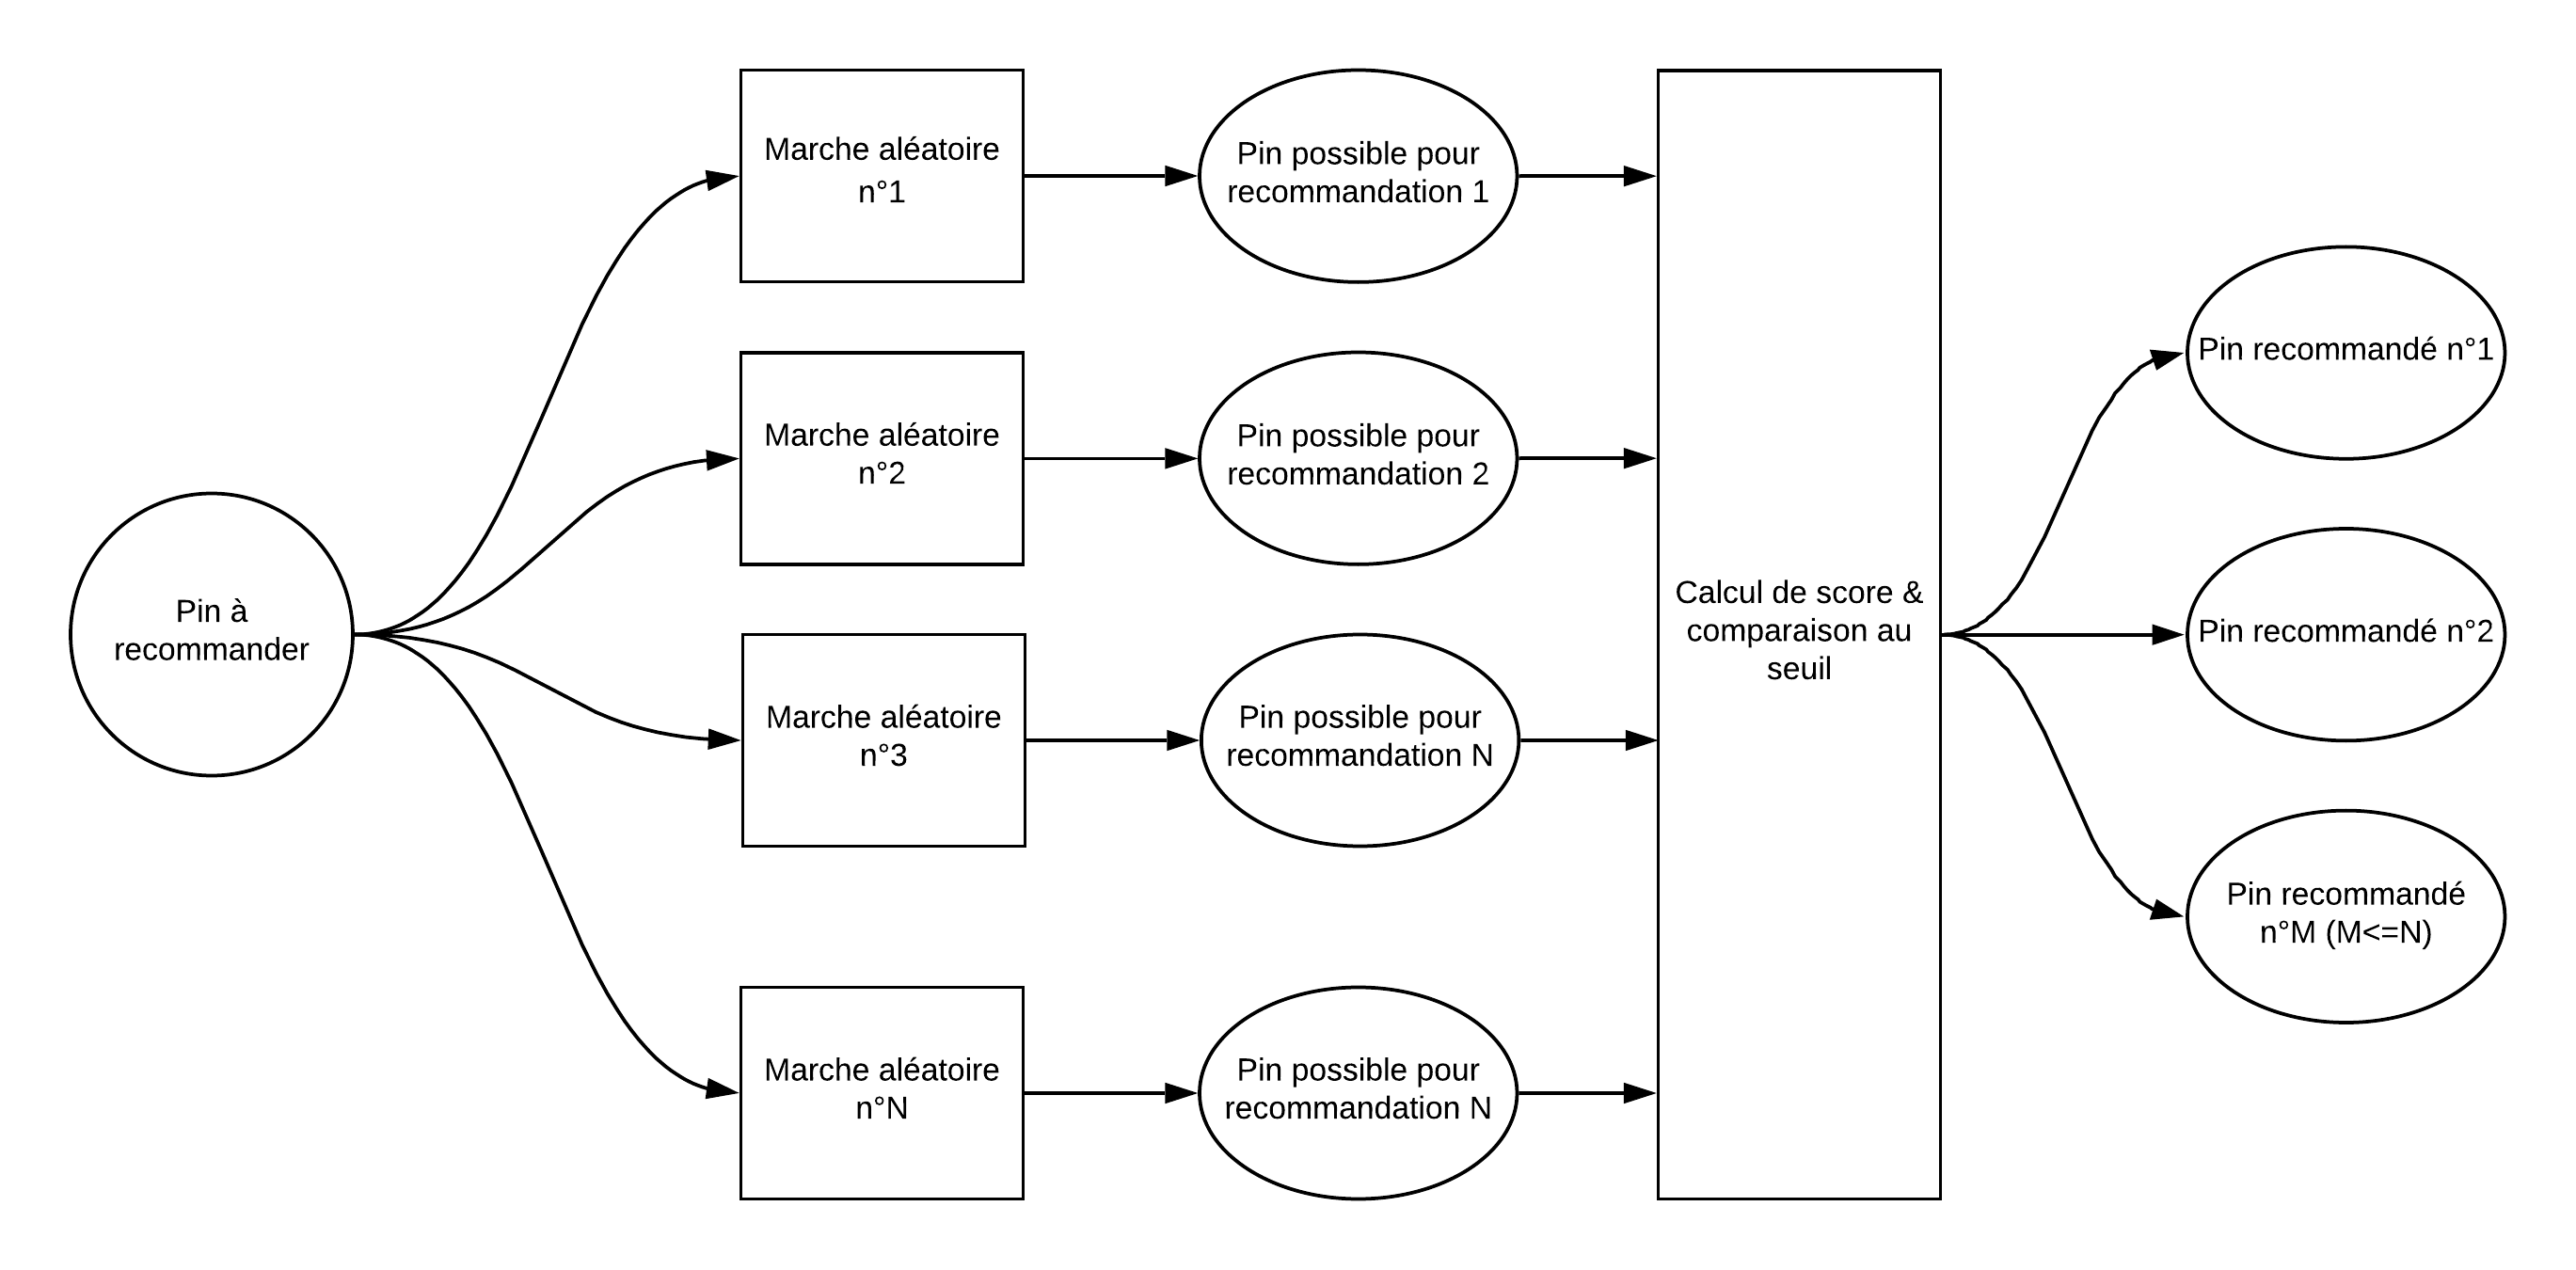
\includegraphics[keepaspectratio = true,scale=0.7]{procpint.png}
	\caption{Heuristique choisie}
	\label{fig:procpint}
\end{figure}

C'est à partir de cette heuristique que j'ai alors implémenté le moteur de recommandation pour Cleep. Cependant, je ne pouvais pas suivre l'ensemble de papier de Pinterest car il y avait quelques limitations en matière de ressources exigées.\\
Pinterest crée son graphe avec une partie de sa base de donnée. Ce sont les pins étant les plus tendances, et les plus vues pendant une période donnée qui y sont inclus, mais aussi les utilisateurs ayant le plus d'interactions avec les autres/ les pins. Le graphe est créé en C++ de manière dynamique. Ainsi le graphe est stocké en mémoire RAM des serveurs, l'heuristique lui est ensuite appliquée. Le graphe est régénérée fréquemment afin d'avoir des recommandations à jour. Ce mode de fonctionnement est un problème car les serveurs de Pinterest coûtent assez cher, ce qui leur permet de faire tenir en RAM des graphes ayant une taille avoisinant le Téraoctet. Cleep ne peut raisonner de la même manière, créer un graphe compilé est donc compliqué. \\

\begin{figure}[!h]
	\centering
	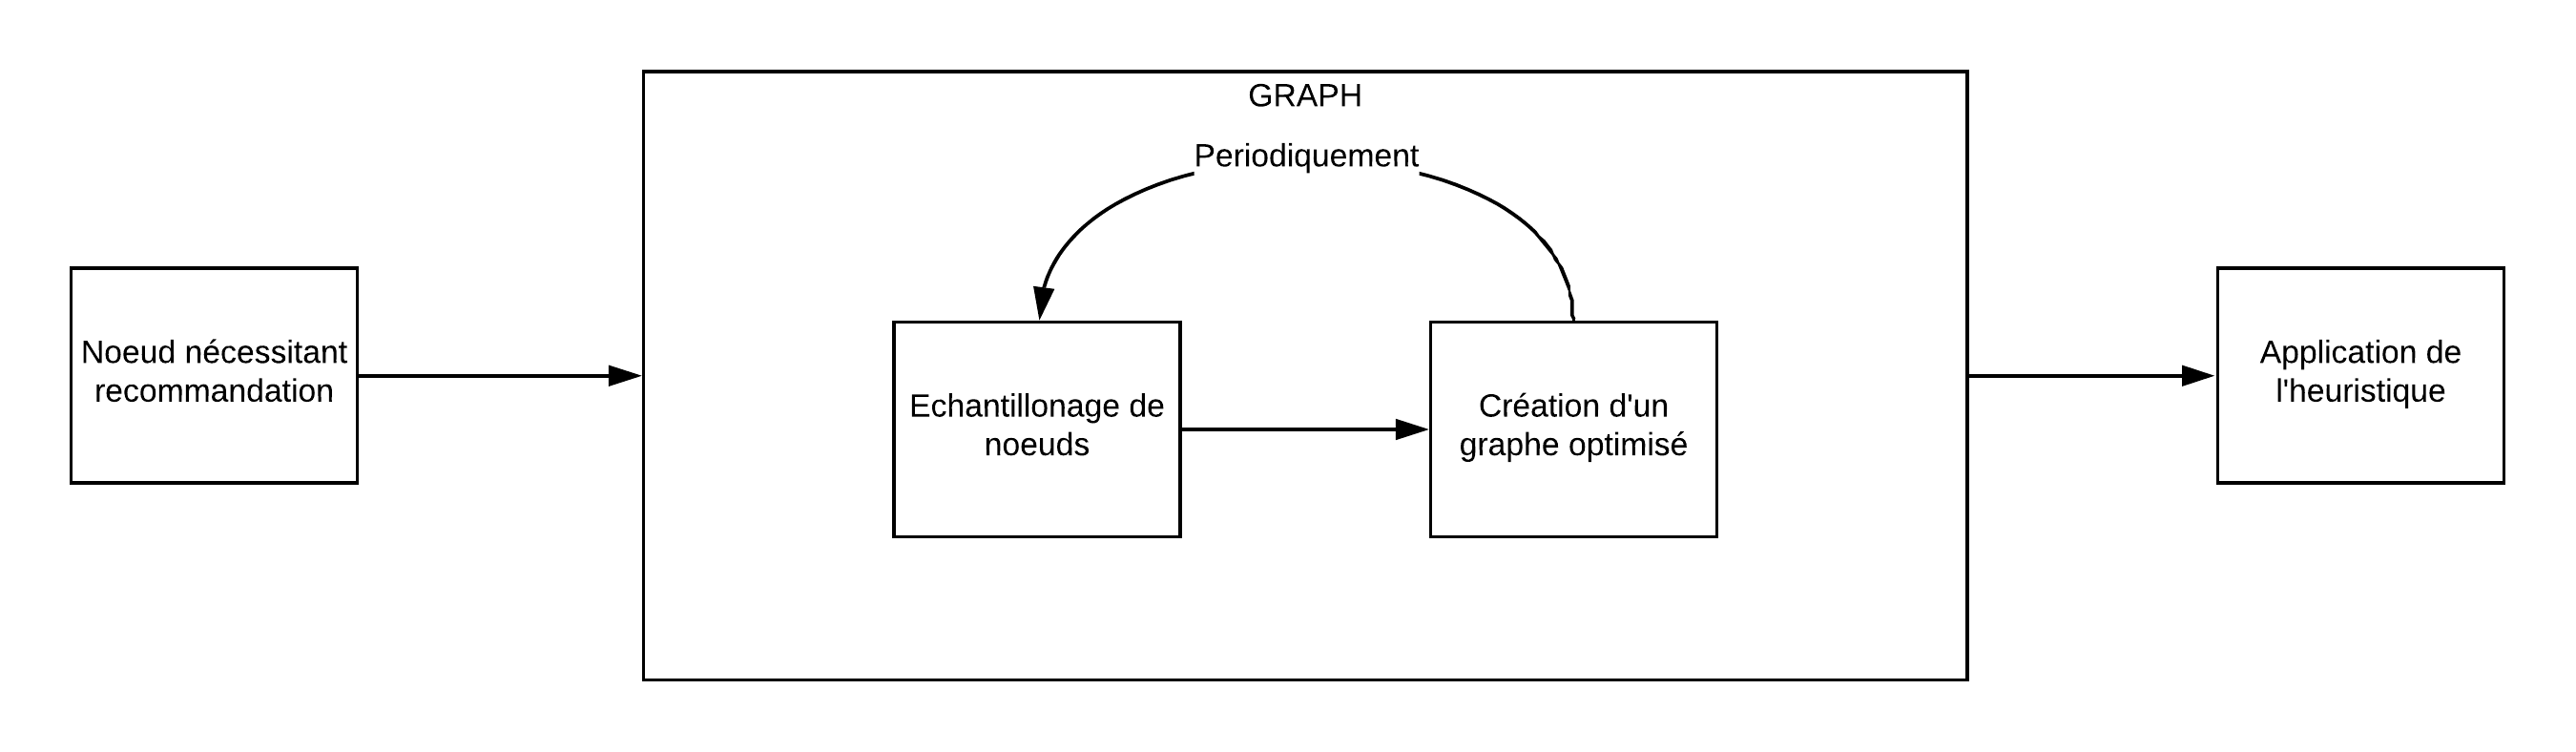
\includegraphics[keepaspectratio = true,scale=0.7]{pintfunc.png}
	\caption{Fonctionnement (simplifié) de Pixie}
	\label{fig:funcpint}
\end{figure}


Par ailleurs la conception d'un graphe avec requêtes optimisés prend beaucoup de temps. Cleep avait besoin d'un moteur de recommandation assez rapidement. Pour ces raisons, il a été choisi de ne pas utiliser un graphe précompilé. C'est ainsi que je me suis tourné vers une solution plus viable : les bases de données en graphe.

\paragraph{Interêt des bases de données en graphe\\}
Les bases de données en graphes, sont une type de base de donnée noSQL dont l'organisation de la donnée repose sur la structure en graphe. Pour rappel, une base de donnée noSQL se caractérise par le fait qu'elle ne se conforme pas aux requêtes SQL, plus particulièrement elle n'est pas conforme au modèle RDBMS (Relational Database Management System).\\
Les définitions suivantes sont spécifiques aux base de données en graphe et peuvent avoir un sens légèrement différent par rapport à l'usage classique en théorie des graphes:
\begin{itemize}
	\itemsep 0 em
	\item Nœud : Entité du graphe contenant de la donnée
	\item Arrête : Entité du graphe reliant deux nœuds pouvant contenir de la donnée 
	\item Collection: Ensemble de nœuds ou arrêtes du même type
	\item Document (plus rare): Informations contenu dans un nœuds (équivalent de document en base MongoDB) 
\end{itemize}
La donnée dans une base noSQL ne suit pas un schéma particulier et peut évoluer rapidement. Ce premier point est très intéressant pour notre cas, car Cleep étant une start-up avec un produit naissant, beaucoup de données sont encore à acquérir pour cerner au mieux les interactions sur la plateforme. Dans le cas d'une base de donnée en graphe, la donnée est souvent stockée au format JSON.\\
En terme de performances, les bases de données graphe repose sur l'index-free adjacency. Dans les bases de données traditionnelles, la recherche d'éléments se fait par recherche d'index. Afin de trouver un élément précis dans une table il faut parcourir l'ensemble des indexes jusqu'à trouver le bon. Cela fait une complexité en $O(n)$ où $n$ est le nombre de donnée dans la table.\\
Dans une base de donnée en graphe, les nœuds n'ont en général pas d'index prédéfini par la bases. Cependant ils ont tout de même une ID qui leur est propre et l'ID de leurs nœuds voisins. Ainsi pour rechercher 1 nœud en particulier dans la base, une base en graphe va agir comme une RDBMS, et faire une comparaison d'ID. Mais ensuite à partir de ce nœud, trouver l'ensemble des nœuds voisins, ou parcourir le graphe selon un certain modèle est en complexité $0(1)$ car l'information est déjà dans le nœud. La \textbf{Figure \ref{fig:indfree}} permet de comprendre ce que cela implique comme changement. Cette caractéristique est l'un des grands avantages de ces bases de données, car cela accélère grandement les requêtes. Dans le cas de Cleep, c'est d'autant plus intéressant que nous cherchons à faire une marche aléatoire sur le graphe. Ce type de base est donc bien adapté au problème.\\
Par ailleurs, les bases de données en graphes sont efficaces en matière de rapidité de requête car les noeuds et arrêtes concernés par la requête sont tous chargés en RAM.\\
Finalement, l'un des derniers problèmes que résolvent les bases de données en graphes, c'est la mise à jour et l'ajout de donné en temps réelles. Dans le modèle relationnel, l'ajout de donnée se fait souvent en batch (plusieurs données ajoutées en même temps), car bien plus rapide. Dans le modèle graphe, seul les noeuds voisins à celui ajouté vont être affecté. D'où la rapidité et la modularité de l'insertion de donnée.\\

\begin{figure}[!h]
	\centering
	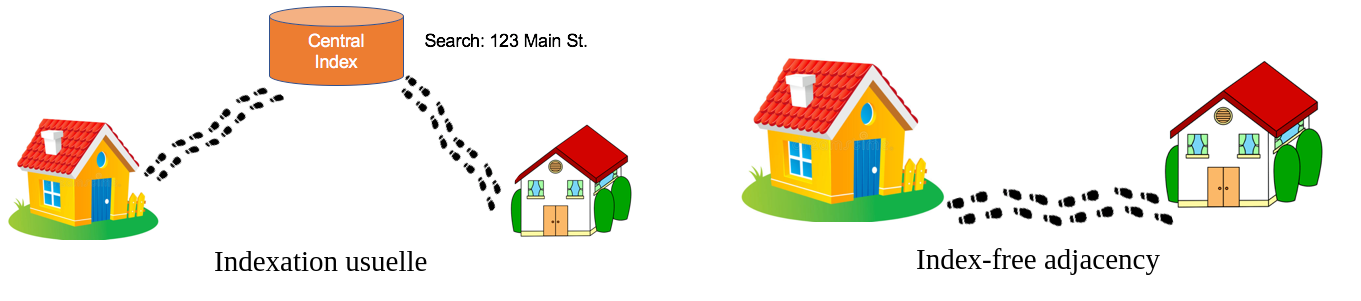
\includegraphics[keepaspectratio = true,scale=0.3]{indfree.png}
	\caption{Principe du index-free adjacency}
	\label{fig:indfree}
\end{figure}

\paragraph{Les désavantages\\}
Les bases de données graphe ont plusieurs défauts qui ont la même origine : la technologie n'est pas encore assez mature:
\begin{itemize}
	\item La plupart des bases de données ont un souci de management de la mémoire. Les très grosses requêtes ont tendance remplir la RAM, et peu de base de données disposent de "spill sur disk" (utiliser la mémoire SDD ou HDD qui possède des cycles bien plus long). Cependant la marche aléatoire chargera très peu de donnée en mémoire RAM par rapport à au seuil critique de "requête lourde". 
	\item Le garbage collector (script dont le but est de libérer l'espace RAM qui n'est plus utilisé) de ces bases de données pose parfois soucis ce qui nous ramène souvent au premier problème
	\item Chaque base de donnée possède son propre langage contrairement aux RDBMS. Contrairement aux bases RDBMS qui utilisent toutes du SQL, le langage de requête n'est pas uniforme. Cela est un grand désavantage car cela force à réinvestir du temps si l'ont veut changer de base de donnée graphe.
	\item Les bibliothèques dans les principaux langages de programmations (python, nodejs ...) sont peu souvent mis à jour et offrent peu de modularité. 
\end{itemize}

Les bases de données en graphe ont qualités et défauts. J'ai jugé que les défauts était négligeable pour le moment par rapport au gain de temps et la "facilité" de developpement qu'offre ce modèle. Par la suite, il fallait donc trouver et étudier le fonctionnement des différentes base de données graphe existantes sur le marché. Selon les recommandations du client, j'ai commencé par étudier la faisabilité du projet sur la base de donnée graphe ArangoDB. En approfondissant mes recherches, et en expérimentant les limites d'ArangoDB, je me suis tourné vers la base graphe la plus utilisée sur le marché : Neo4j.

\paragraph{Comparatif ArangoDB / Neo4j\\}
J'ai réalisé plusieurs tests comparatifs entre ArangoDB et Neo4j. Je présenterai ici que les résultats. J'approfondirai cette partie dans la prochaine sous-section. ArangoDB et Neo4j sont assez différentes dans leur manière d'envisager les bases de données en graphe.\\
ArangoDB est une base de donnée qui reprend beaucoup d'élément de mongoDB, en organisant ses données selon des collections et des documents. Ainsi ArangoDB propose une indexation qui permet de récupérer les éléments de manière plus rapide (identifié par leur collection. Le modèle graphe n'est donc pas le seul que propose ArangoDB (le modèle key-value et document sont aussi présents). A l'inverse, Neo4j ne propose qu'un seul type de modèle, celui en graphe, mais le moteur derrière se retrouve plus optimisé que celui d'ArangoDB.\\

L'un des grands avantages de Neo4j est sa documentation (bien qu'encore assez sommaire) vis à vis des algorithmes développés pour la traversée de graphe \cite{neo4j}. Cette base de donnée possède certains algorithmes de traversée qu'il est possible d'appeler directement via son langage de requête (Cypher). En particulier, il y a une version optimisé pour neo4j de la marche aléatoire. A l'inverse, ArangoDB ne possède pas d'algorithmes de traversé inclus originellement, ce qui nous oblige à les créer par nous même. Les tests comparatifs que j'ai effectué montre justement que les performances de la marche aléatoire d'ArangoDB développé par moi même sont inférieurs par rapport à celle de Neo4j en terme de temps d'execution et de mémoire RAM consommé.\\
Après discussion avec le client sur la marche à suivre et l'ensemble du travail réalisé jusque là, nous nous sommes mis d'accord sur l'utilisation de l'heuristique de Pinterest avec Neo4j comme support pour le graphe.

\subsubsection{Implémentation}
L'implémentation de l'heuristique de Pinterest adapté au problème de Cleep a pris du temps, notamment pour des raisons techniques (manque de documentation sur l'utilisation de Neo4j, les API/wrappers dans les autres langages ne fonctionnant pas ...), mais aussi pour des raisons de conceptions. L'implémentation s'est divisée en trois étapes :
\begin{itemize}
	\item Adaptation sur Neo4J, instanciation des serveurs, création des plu-gins adaptés et première version simple d'un moteur de recommandation
	\item Études des améliorations en particulier au niveau de la fonction de scoring (qui permet d'évaluer la qualité d'une recommandation)
	\item Tests de la première version du moteur
\end{itemize}

Avant de commencer cette partie, vous pouvez retrouver en \textbf{Annexe 9.3} de l'heuristique que j'ai implémenté par la suite. 

\paragraph{Première version du moteur de recommandation\\}
Tout d'abord, l'ensemble des données que possède Cleep est stocké dans une base mongoDB. Le problème est qu'il n'est pas possible de réaliser un simple dump de base. En effet, seule les informations concernant les cleeps, les utilisateurs, les listes de cleeps et les relations nous intéresse. Donc la première étape a été d'établir les données utiles qui allaient composer la base de donnée de Neo4j.\\
Par ailleurs, pour créer et tester un moteur de recommandation fonctionnel, je ne nécessitais la base en entière. En effet je pouvais commencer à développer en local avec une base de donnée factice afin d'expérimenter. Ainsi, avec le client nous nous sommes mis d'accord sur le format des données à utiliser (ie comment ils seront enregistrés dans la base) et j'ai commencer l'implémentation.\\
En premier lieu j'ai créé un script permettant de générer les données nécessaires et de commencer l'implémentation du moteur de recommandation. Le paragraphe suivant permet de comprendre ce que contient la base de donnée ce qui va être utile pour l'étude de la fonction de scoring. Le format des données est le suivant:\\
Noeud cleep :
\begin{itemize}
	\item Nom de domaine du Cleep
	\item Devise du produit
	\item Prix du produit
	\item Tags fournis par google vision
	\item Date de création
	\item Statut du cleep : actif ou archivé par l'utilisateur
\end{itemize}

Noeud utilisateur:
\begin{itemize}
	\item Genre de la personne
	\item Âge de la personne
	\item Nombre d'activités vis à vis d'un domaine et date de la dernière activité. Les activités peuvent être : la création d'un cleep, la vue d'un cleep, l'ajout d'un like à un cleep, la copie d'un cleep où l'action d'aller sur le site original du cleep. 
\end{itemize}

Noeud Listing:
\begin{itemize}
	\item Statut de la liste : active ou archivée par l'utilisateur
	
\end{itemize}
Relation utilisateur $\leftrightarrow$ cleep:
\begin{itemize}
	\item Nombre d'activité d'un utilisateur sur le cleep relié et la date de dernière activité. Les activités peuvent être : la création d'un cleep, la vue d'un cleep, l'ajout d'un like à un cleep, la copie d'un cleep où l'action d'aller sur le site original du cleep.
\end{itemize}

Relation utilisateur $\leftrightarrow$ listing:
\begin{itemize}
	\item Nombre d'activité d'un utilisateur sur la liste reliée et la date de dernière activité. Les activités peuvent être : la vue d'une liste ou l'action de suivre la liste.	
\end{itemize}

Relation cleep $\leftrightarrow$ listing: il n'y pas de donnée particulière sur cette relation.\\

Pendant la première partie de l'implémentation, j'ai donc travaillé avec une base factice composé de ces éléments. Comme énoncé précédemment, Neo4j possède un algorithme de marche aléatoire qui peut être appelé directement par son langage de requête : Cypher \cite{cypher}. Cette algorithme permet donc de retourner à partir d'un cleep, un chemin aléatoire. Il prend plusieurs paramètres en entré dont deux primordiaux : le nombre de marches aléatoire à faire et la profondeur de la marche aléatoire.\\
Le problème est que le dernier nœud d'une marche aléatoire n'est pas toujours un cleep. De plus, la requête retourne uniquement les ID des nœuds et pas le chemin en entier avec les données associés. Une autre requête est donc nécessaire pour avoir les chemins en entiers.\\
Cependant Neo4j offre la possibilité de développer des plu-gins Java qui peuvent être aussi appeler pendant une requête. Ainsi deux solutions étaient possibles :
\begin{itemize}
	\item Effectuer deux requêtes pour récupérer les chemins en entiers et ensuite traiter les chemins pour avoir une score.
	\item Effectuer une seule requête retournant les cleeps recommandé via le développement d'un plu-gin.
\end{itemize}
J'ai choisi la deuxième solution, car cela permettait d'éliminer une requête dans le processus et ainsi réduire le temps total d'exécution. 
\newpage
\paragraph{Description du processus\\}
Le but maintenant de savoir comment créer le plu-gin afin de pouvoir appliquer un score sur le chemin. Il existe différents type de plu-gin Java pouvant être créé sur Neo4j. Ce qui nous intéresse sont les plu-gins d'agrégation \cite{aggrg}. La marche aléatoire sous Neo4j fonctionne de manière séquentielle, elle ne ressort pas directement un chemin mais les nœuds un par un. La fonction de score doit donc être capable de garder en mémoire un certain nombre de paramètre et d'appliquer un score à chaque étape de la marche aléatoire. C'est pourquoi les plu-gins d'agrégation sont adaptés à ce problème.\\
La figure suivante (\textbf{\ref{fig:algo}}) décrit le processus global pour appliquer un score et avoir une recommandation.
\begin{figure}[!h]
	\centering
	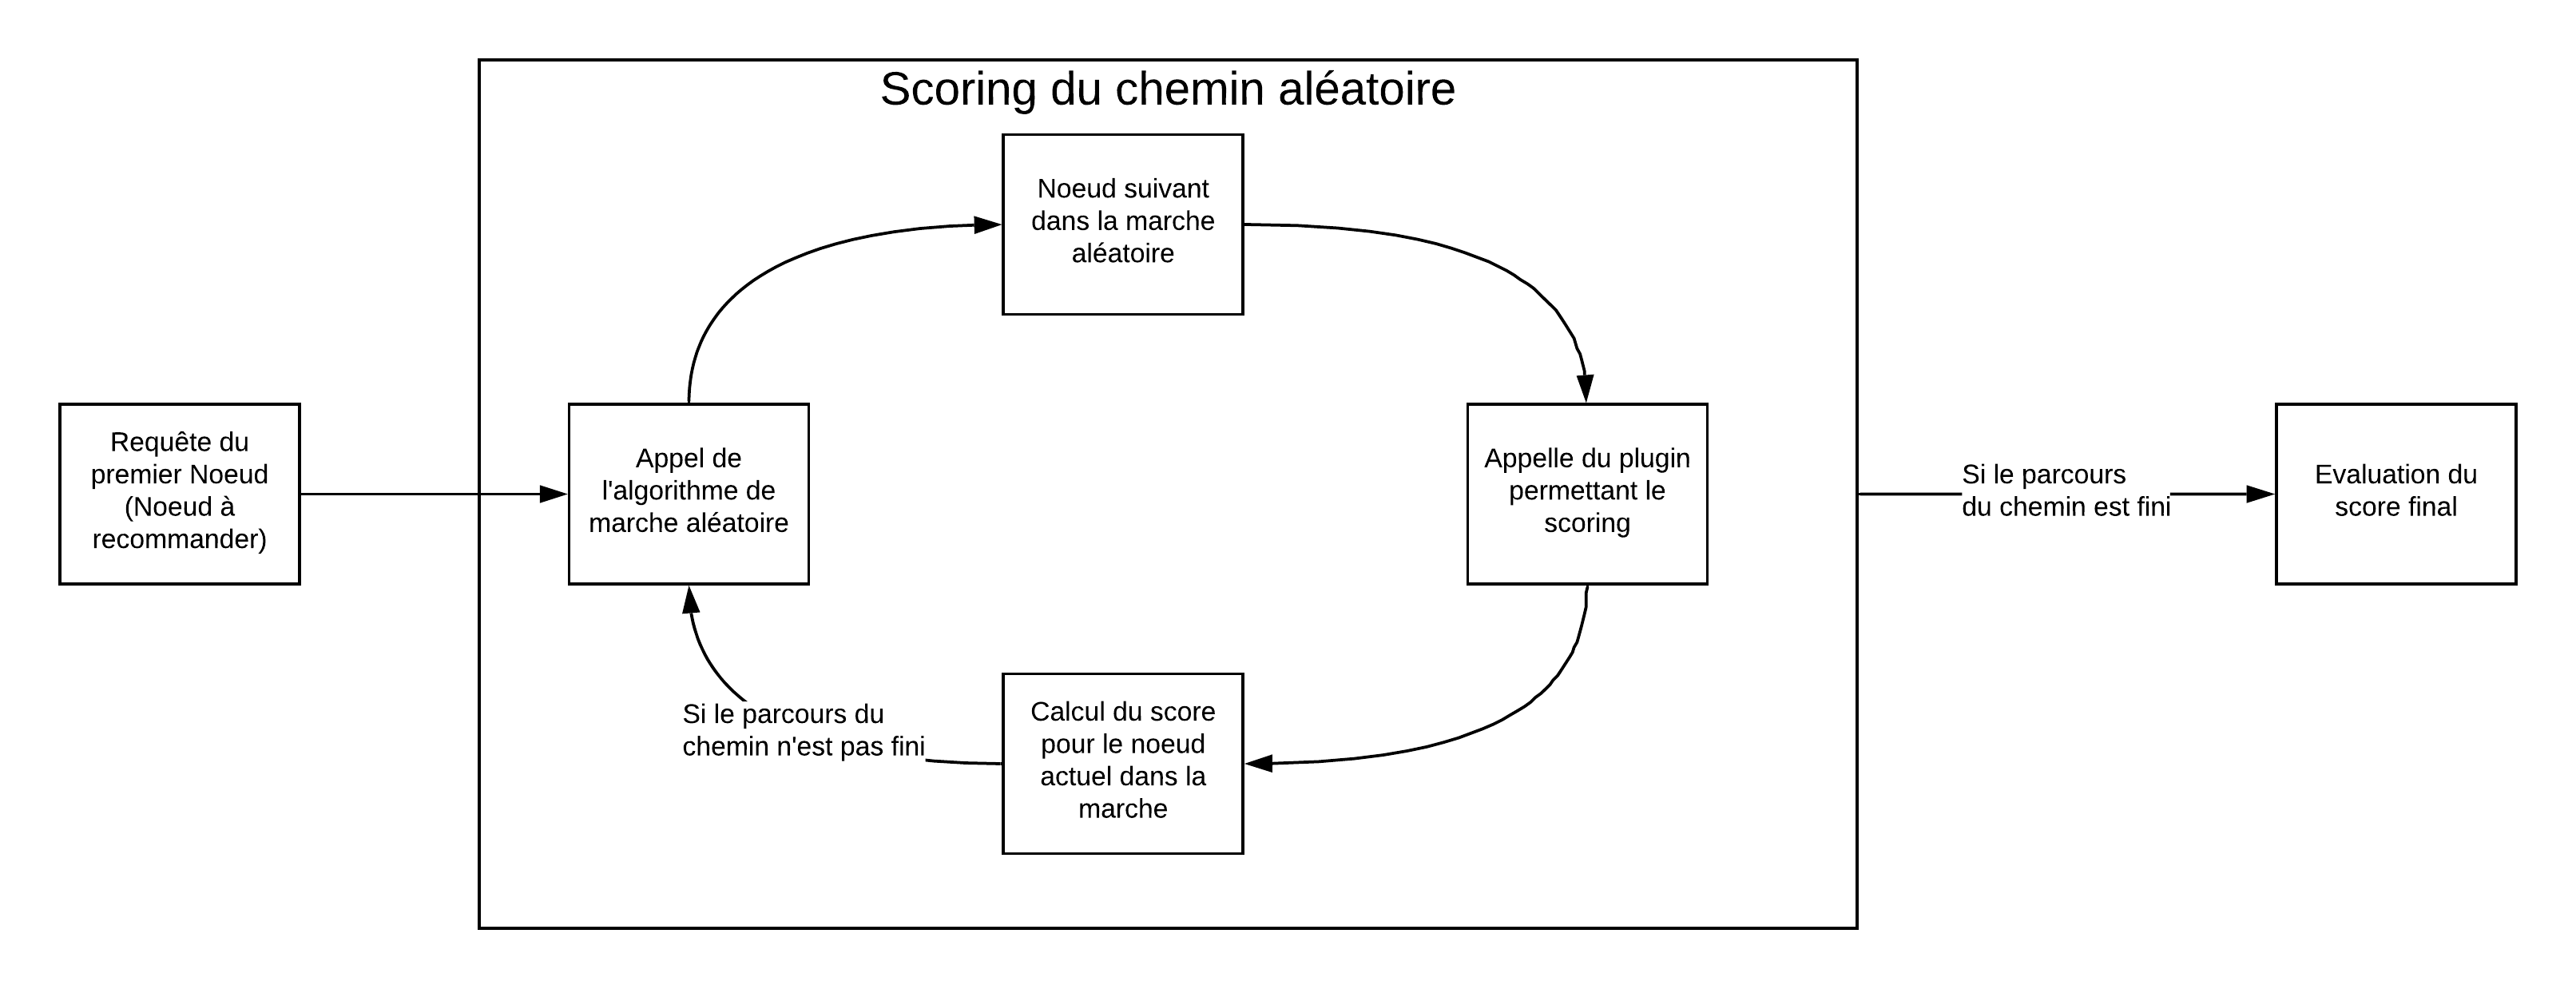
\includegraphics[keepaspectratio = true,scale=0.7]{proccleep.png}
	\caption{Processus pour appliquer un score}
	\label{fig:algo}
\end{figure}

Le processus étant défini, il reste la fonction de scoring à décrire. 

\paragraph{Fonction de scoring\\}
\subparagraph{1ère version\\}
La première version de la fonction de scoring était assez sommaire, dans le sens que mon but était de montrer que j'avais mis l'architecture en place et qu'il est possible de faire un scoring complexe utilisant toutes les données.\\
Tout d'abord le score est normalisé entre 0 et 1. Plus le score est proche de 1, plus le cleep est à recommander, et inversement quand le score est proche de 0. Ce qui suit présente les différents calculs effectué à chaque étape de la fonction de scoring. Cette fonction prend donc en entrée, le cleep original, le nœud sur lequel vient de s'arrêter la marche aléatoire et le nœud le précédent ainsi que les relations qui en découlent. Pour rappel, la fonction de scoring est une fonction d'agrégation qui calcul un score pour chaque nœud de la marche\\

Pour les relations contenant des activités (ie cleep $\leftrightarrow$ user), et les activités utilisateur : un coefficient est associé. Ce dernier est plus ou moins grand en fonction de l'activité. Par ailleurs une deuxième donnée est disponibles pour les activités : le nombre d'interaction avec l'activité. Ce nombre d'interaction est normalisé avec la fonction (\ref{eq:1}) et multiplié au coefficient :
\begin{equation}
\label{eq:1}
f(x) = \frac{atan(1/factor \times x)}{\pi/2} \hspace{1cm} \mbox{ \vbox{\noindent où $x$ est le nombre d'interacitons \\$factor$ est le facteur de normalisation }}
\end{equation}
Ainsi pour chaque activité la formule suivante est utilisée:
\begin{equation}
\label{eq:2}
s_{act} = coefficient\times\frac{atan(1/factor \times x)}{\pi/2} \hspace{1cm} \mbox{\vbox{\noindent $x$ est le nombre d'interacitons, \\$factor$ est le facteur de  normalisation \\ $coefficient$ le coefficient relié à l'activité}} 
\end{equation}
C'est cette formule que j'ai décidé de garder car elle permet de prendre en compte les différences entre les activités et d'adapter le poids de ces dernières dans le score. J'ai utilisé cette fonction de normalisation car j'avais besoin d'une injection $\mathbb{N} \rightarrow [0;1]$ (\textbf{\ref{fig:atan}}). 
\begin{figure}[!h]
	\centering
	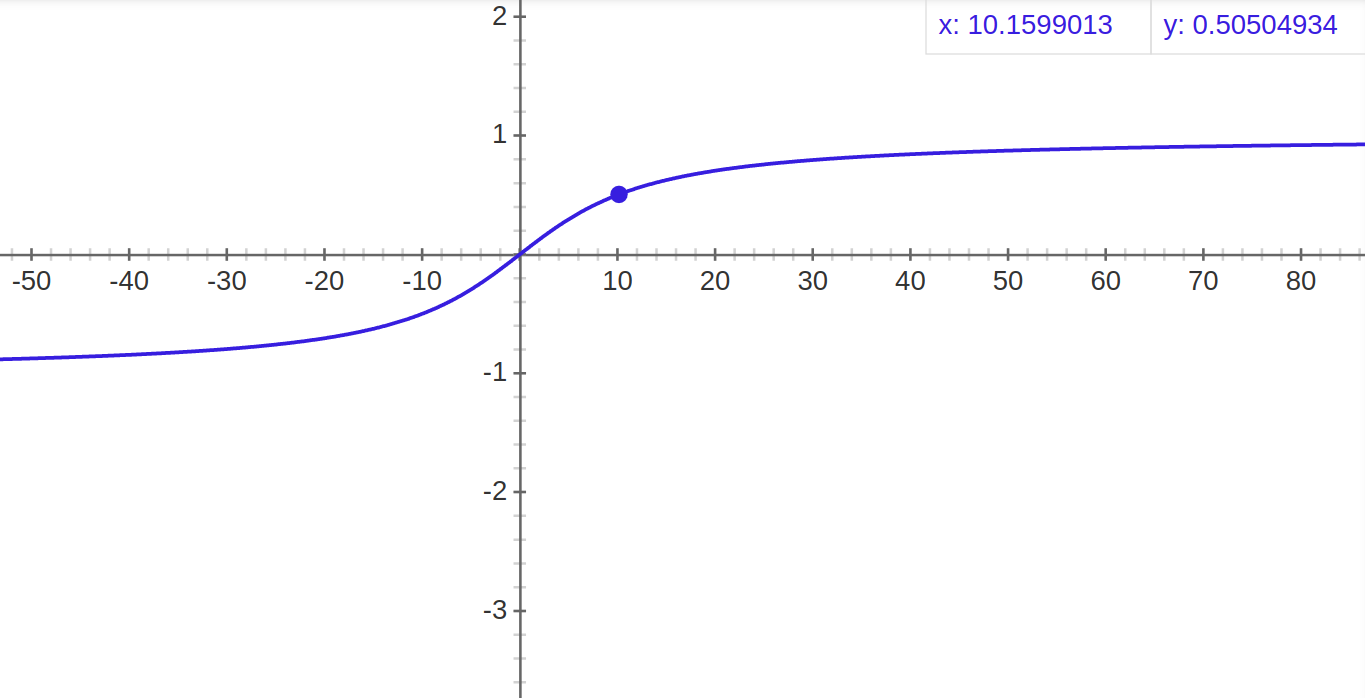
\includegraphics[keepaspectratio = true,scale=0.3]{atan.png}
	\caption{Fonction de normalisation}
	\label{fig:atan}
\end{figure}

De plus il est possible de contrôler la mi-valeur de cette fonction avec $factor$. Les deux inconnus à déterminer pour chaque activités sont donc $coefficient$ et $factor$. $factor$ est une variable assez facile à déterminer, le but est de savoir à partir de quelle valeur, on considère nous sommes dans la moyenne d'interaction. Ainsi j'ai calculé via des requêtes Cypher la moyenne pour chaque activité ce qui m'a donné les valeurs de $factor$. La manière de trouver les valeurs de $coefficient$ est empirique et sera décrit dans la partie test. Ainsi pour chaque activité est retournée une valeur $s_act$.\\

Concernant les données utilisateurs, si l'utilisateur a eu des interactions avec le cleep original, alors un bonus de 10\% est donné au score.\\

Concernant les données de cleep, c'est la différence de prix entre le cleep original et le cleep actuel qui va jouer avec cette formule (\ref{eq:3}):
\begin{equation}
\label{eq:3}
s_{price} = coefficient\times\frac{atan(1/factor \times |price_{cur} - price_{original}| )}{\pi/2} \hspace{1cm} \mbox{\vbox{\noindent $price_{cur}$ est prix du cleep actuel,\\ $price_{original}$ le prix du cleep original \\ $factor$ est le facteur de normalisation \\ $coefficient$ le coefficient relié à l'activité}}
\end{equation}
De plus si les deux cleeps proviennent du même domaine, alors un bonus de 10\% est donné au score. Finalement les tags google vision sont pris en compte selon la formule suivante:
\begin{equation}
\label{eq:4}
s_{vision} = coefficient\times \frac{\sum_{t \in tags}c_{t}}{n_{t}}
\hspace{1cm} \mbox{\vbox{\noindent $coefficient$ le coefficient relié au google tag vision\\
$tags$ est l'ensemble des tags communs au cleep orignal et actuel\\
$c_{t}$ est le taux de confiance par rapport au tag\\
$n_{t}$ est le cardinal de $tags$ (ie le nombre de tags en commun)}}
\end{equation}
\newpage
Une fois ces scores intermédiaire calculés, une moyenne pondéré par les coefficient est calculée que l'on nomme $s_{mean}$, ce qui nous donne un résultat entre 0 et 1. Le score final pour cette étape du chemin aléatoire est alors donnée par la formule suivante :
\begin{equation}
\label{eq:4}
score = \frac{s_{mean} + score}{2}
\hspace{1cm} \mbox{\vbox{\noindent $score$ est le score calculé à l'étape précédente}}
\end{equation}

Cette première version de la fonction de scoring a permis de fournir une première version fonctionnelle du moteur de recommandation. Plusieurs améliorations ont par la suite été apporté, cependant la base restera la même, notamment en matière de calcul des scores intermédiaires.

\subparagraph{2ème version\\}
La deuxième version moteur de recommandation inclut un troisième type de noeud : les listes de cleep. Jusqu'à présent je travaillais uniquement avec les nœuds cleep et utilisateurs afin de produire rapidement un moteur de recommandation. Pareillement, les activité liés aux listes seront calculé de la même manière. De plus si le cleep orignal appartient à la liste étudiée et si la liste étudiée n'appartient pas à l'utilisateur qui demande la recommandation,  alors un bonus de 10\% est donné au score. De même si le cleep original et un cleep étudié lors de la marche aléatoire sont dans la même liste, un bonus de 10\% est donné au score. Ces bonus sont attribué, car les listes créées par les utilisateurs sont sensées regrouper des cleeps de même catégorie, donc des cleeps qui ont de forte chance d'être recommandable.\\

J'ai intentionnellement homis plusieurs détails dans le développement du moteur de recommandation afin de ne pas alourdir la lecture du rapport. Notamment les erreurs de conceptions vis à vis du scoring, mais aussi vis à vis du fonctionnement de la base de donnée.

\paragraph{Tests du moteur\\}
Le moteur de recommandation est passé par plusieurs phase de tests. Tout d'abord la phase préliminaire de tests entre le client et moi même. Pour chaque modification effectué sur le moteur de recommandation, nous testions le moteur de recommandation avec des tests unitaire développé pour. Ces derniers testait le fonctionnement attendu selon les différents cas possible. Par exemple, un chemin $cleep \leftrightarrow cleep$ n'est pas possible et donc doit retourner une erreur. Un chemin $cleep \leftrightarrow utilisateur \leftrightarrow cleep$ doit ou les deux cleeps sont le cleep original doit retourner une "NaN" value, vu que le chemin ne donne aucune recommandation possible. L'ensemble de ces tests permettent de vérifier si le moteur de recommandation fonctionne comme il a été pensé.\\
Au sujet des coefficients, leur valeurs ont d'abord été évalué par moi en essayant de ne pas être aberrant. Par exemple le coefficient lié à la vue d'un cleep est bien moins grand que le coefficient lié au partage d'un cleep vu que l'action de partager est plus rare et engage plus l'utilisateur. Par la suite afin de raffiner la valeur de ces coefficients, une réunion interne à Sia Partners et Cleep a été organisée.\\
Finalement une phase d'A\&B testing a été lancé pour voir si le moteur de recommandation est efficace. Le principe est de proposer à une base d'utilisateur l'application avec le moteur de recommandation et une autre base d'utilisateur l'application sans moteur de recommandation (ie avec des recommandations proposé au hasard). Si les utilisateurs avec le moteur de recommandation suivent plus les recommandations, alors le moteur est efficace sinon il ne l'est pas. Durant le développement du moteur, j'ai aussi intégré une interface de log, permettant de comprendre pourquoi certaines recommandations ne marchent pas et pourquoi d'autres fonctionnent. Je ne suis pas resté assez longtemps pour avoir les résultats de l'A\&B testing, cependant à la suite de ce dernier, les coefficients auraient une nouvelle fois changé pour être plus adapté aux actions de la population de Cleep.

\subsection{Vision critique et apport personnel}
Dans cette partie, je reviens sur quelques éléments apparus au cours du développement du moteur de recommandation qui demandent un peu plus d'approfondissement.


\paragraph{Tests sur ArangoDB et Neo4j\\}
Afin de comparer les deux bases de donnée, j'ai effectué plusieurs tests comparatifs sur les bases de données notamment en terme de temps d'exécution d'une marche aléatoire. L'étude a été réalisé en local, et donc avec une RAM limité.\\
Ainsi les tests ont été réalisé sur une base de donnée contenant 500 utilisateurs, 10.000 cleeps et 1.4 millions de connexions. J'ai délibérément ignorer les listes pour rendre les tests plus léger et moins compliquer à mettre en place. En effet pour avoir une idée du temps d'exécution et du temps de requête assez proche de ce qu'on allait avoir en production, des bases avec des données factices ont été générée. Le but étant d'avoir des nœuds et des arrêtes contenant des données comme c'est le cas pour Cleep.\\
L'étude étant réalisée sur la marche aléatoire, il y a trois paramètres sur chaque graphe: 
\begin{itemize}
	\item Number walker : Nombre de marche aléatoire faites
	\item Depth : La profondeur de la marche aléatoire (ie le nombre d'étape faite pendant la marche)
	\item Time : Le temps médian d’execution. Pour chaque couple (number walker, depth) 100 réalisations ont été effectuées et la médiane est prise comme référence
\end{itemize} 
Les figures suivantes montrent la comparaison entre les deux solutions. Des graphes supplémentaires sont disponibles en \textbf{Annexes 9.2}.

\begin{figure}[!h]
	\centering
	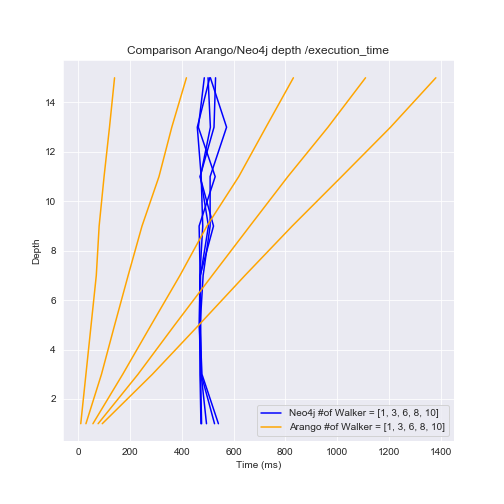
\includegraphics[keepaspectratio = true,scale=0.7]{comparison_depth_time.png}
	\caption{Comparaison des bases en fonction de la profondeur et du temps médian}
	\label{fig:depthtime}
\end{figure}

Les figures suivantes montrent la comparaison entre les deux solutions. Des graphes supplémentaires sont disponibles en \textbf{Annexes 9.2}. Ces graphes représentent les même résultat mais de manière séparé (et un peu plus lisible) pour chaque base de donnée.
De ces deux graphes (\textbf{figure \ref[fig:depthtime]} \& \ref{fig:walker}), deux conclusions peuvent être tirées:
\begin{itemize}
	\item Le temps d’exécution pour arangoDB de la marche aléatoire est plus lente dès qu’on augmente le nombre de walkers ou la profondeur.
	\item Le temps d’exécution pour Neo4j de la marche aléatoire semble être constant. La moyenne de 500 ms qu’on peut voir sur tout les graphes (ceux en Annexes inclus) est peut être biaisé par la puissance de la machine sur laquelle j'ai effectué le test. Il est possible que sur un serveur le temps de traitement soit moins long. Cela indiquerait donc que Neo4j est plus gourmand en ressources.
\end{itemize}

\begin{figure}[!h]
	\centering
	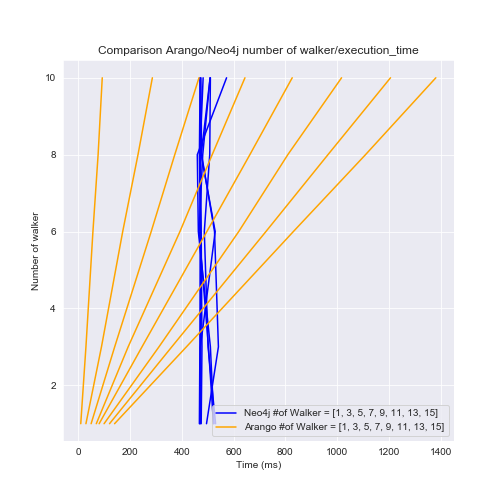
\includegraphics[keepaspectratio = true,scale=0.7]{comparison_nbWalker_time.png}
	\caption{Comparaison des bases en fonction du nombres de chemin aléatoire et du temps médian}
	\label{fig:walker}
\end{figure}

Par ailleurs ces tests ne prennent pas en compte la latence dû à la connexion au serveur. Ici le travail a été fait en local, cette latence est nulle. Cependant, dans le cas de Neo4j, l’ensemble de la marche aléatoire est effectuée en une requête. Dans le cas d’ArangoDB, le nombre de requête est de l’ordre de $O(depth\times number of walker)$, ce qui peut être problématique en terme de latence.\\
Cette différence s'explique par le fait que j'ai du créer moi même l'algorithme de marche aléatoire pour ArangoDB. Avec ce dernier, le passage au noeud suivant dans la marche aléatoire implique à chaque fois une nouvelle requête.  J'ai été en contact avec les développeurs travaillant sur ArangoDB. Ces derniers m'ont confirmé que l'algorithme que j'avais développé était la seule manière de faire pour le moment car ArangoDB gère très mal la sélection aléatoire de nœuds.\\

Sachant que dans le cas de Cleep, le nombre de marche faite pour recommander un nœud sera important (vu que nous faisons des marches aléatoires jusqu'à l'obtention d'un assez grand nombre de cleep recommandés). De même la profondeur est un paramètre qui peut aussi devenir grand en fonction de la qualité des cleeps que ressort le moteur de recommandation. Si les cleep proches sont de "bonnes qualité", alors il n'est pas nécessaire d'aller en profondeur, cependant si cela n'est pas le cas, le paramètre peut augmenter. Pour toute ces raisons Neo4j a été choisi par rapport à ArangoDB.

\newpage
\paragraph{Amélioration de la marche aléatoire de Neo4j\\}
Contrairement à ArangoDB, la marche de Neo4j est efficace en terme de temps d'exécution. Ce dernier provient d'une procédure développé par l'équipe de Neo4j, dont le code est disponible en open-source.\\
En réalisant les tests sur les dernières version du moteur de recommandation, je me suis rendu compte que la marche aléatoire suivait bien un mouvement Brownien (ce qui en soit est le principe de la marche aléatoire) car le moteur de recommandation retournait souvent les mêmes cleeps. Et en regardant les chemins dans l'interface de debug, j'ai remarqué que les cleeps recommandés étaient les cleeps voisins du cleep original. Cela pose problème car nous n'avons plus la diversité dans nos recommandations car nous sommes limités à une échantillon des possibles.\\
Afin de résoudre ce problème, j'ai modifier la procédure qu'utilisait Neo4j pour faire la marche aléatoire. J'ai fait en sorte que cette marche pseudo-aléatoire ait plus de chance de s'éloigner du cleep d'origine, que de s'en approcher. Les tests après implémentations de cette nouvelle caractéristique montrent bien l'éloignement des marches aléatoires, et il est plus rare de retomber plusieurs fois sur le même cleep.

\paragraph{Optimisation du calcul de score\\}
Le calcul de score dépend grandement du chemin parcouru. En effet, selon le chemin, les cleeps, listes et utilisateurs qui le composent peuvent être différents et donc fournir des résultats différents. Cependant avec la marche aléatoire il arrive souvent de faire une boucle (\textbf{firgure \ref{fig:boucle}}). Le problème dans cet exemple est que la boucle va impacter le score (que ce soit négativement ou positivement). Le score du chemin 1 $\rightarrow$ 2 $\rightarrow$ 3 $\rightarrow$ 4 impacte le score du chemin 5 $\rightarrow$ 6. Ce qui nous intéresse c'est le chemin du cleep \#1 au cleep \#3 sans revenir sur son chemin car ca n'a pas grand interêt pour la recommandation.\\
En effet, avec une boucle il est possible de recommander n'importe quel cleep, en faisant une boucle qui ait un impact très positif. Par ailleurs, on s'éloigne aussi de la notion de proximité et de distance dans le graphe : dans l'exemple, le cleep \#2 a autant d'influence sur le score que le cleep \#3.\\
La solution adaptée est la suivante:
\begin{itemize}
	\item L'état des variables nécessaire au fonctionnement de l'algorithme est enregistré à chaque étape
	\item Au début de la boucle un état $E_{1}$ est enregistré
	\item A la fin de le boucle cet l'état $E_{1}$ devient l'état actuel de l'algorithme
\end{itemize}

\begin{figure}[!h]
	\centering
	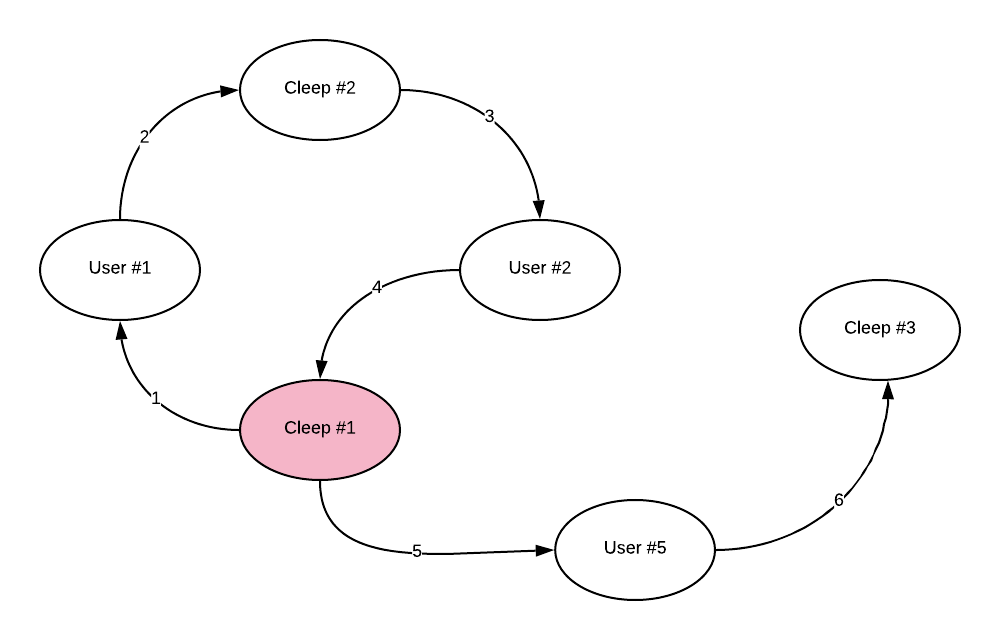
\includegraphics[keepaspectratio = true,scale=0.7]{boucle}
	\caption{Boucle chemin aléatoire}
	\label{fig:boucle}
\end{figure}
\newpage
Ainsi les boucles n'ont pas d'impact sur la procédure adapté. Plusieurs cas particuliers de relations se sont aussi imposés comme des boucles (la \textbf{figure \ref{fig:bbb}} explicite le terme de boucle conditionné par une relation):
\begin{itemize}
	\item cleep $\rightarrow$ user : où l'utilisateur est le propriétaire du cleep. A l'inverse la relation user $\rightarrow$ cleep où l'utilisateur est le propriétaire du cleep n'est pas considéré comme une boucle. Dans le premier cas on considère que le chemin aléatoire n'avance pas car il retourne vers le propriétaire d'un cleep et le but du moteur est de recommander des cleeps et non des utilisateurs. C'est pourquoi le second cas n'est pas considéré comme une boucle.
	\item cleep $\rightarrow$ liste : où la liste possède le cleep. (même justification que pour cleep $\rightarrow$ user)
	\item User  $\rightarrow$  liste et liste  $\rightarrow$  User
\end{itemize}

\begin{figure}[!h]
	\centering
	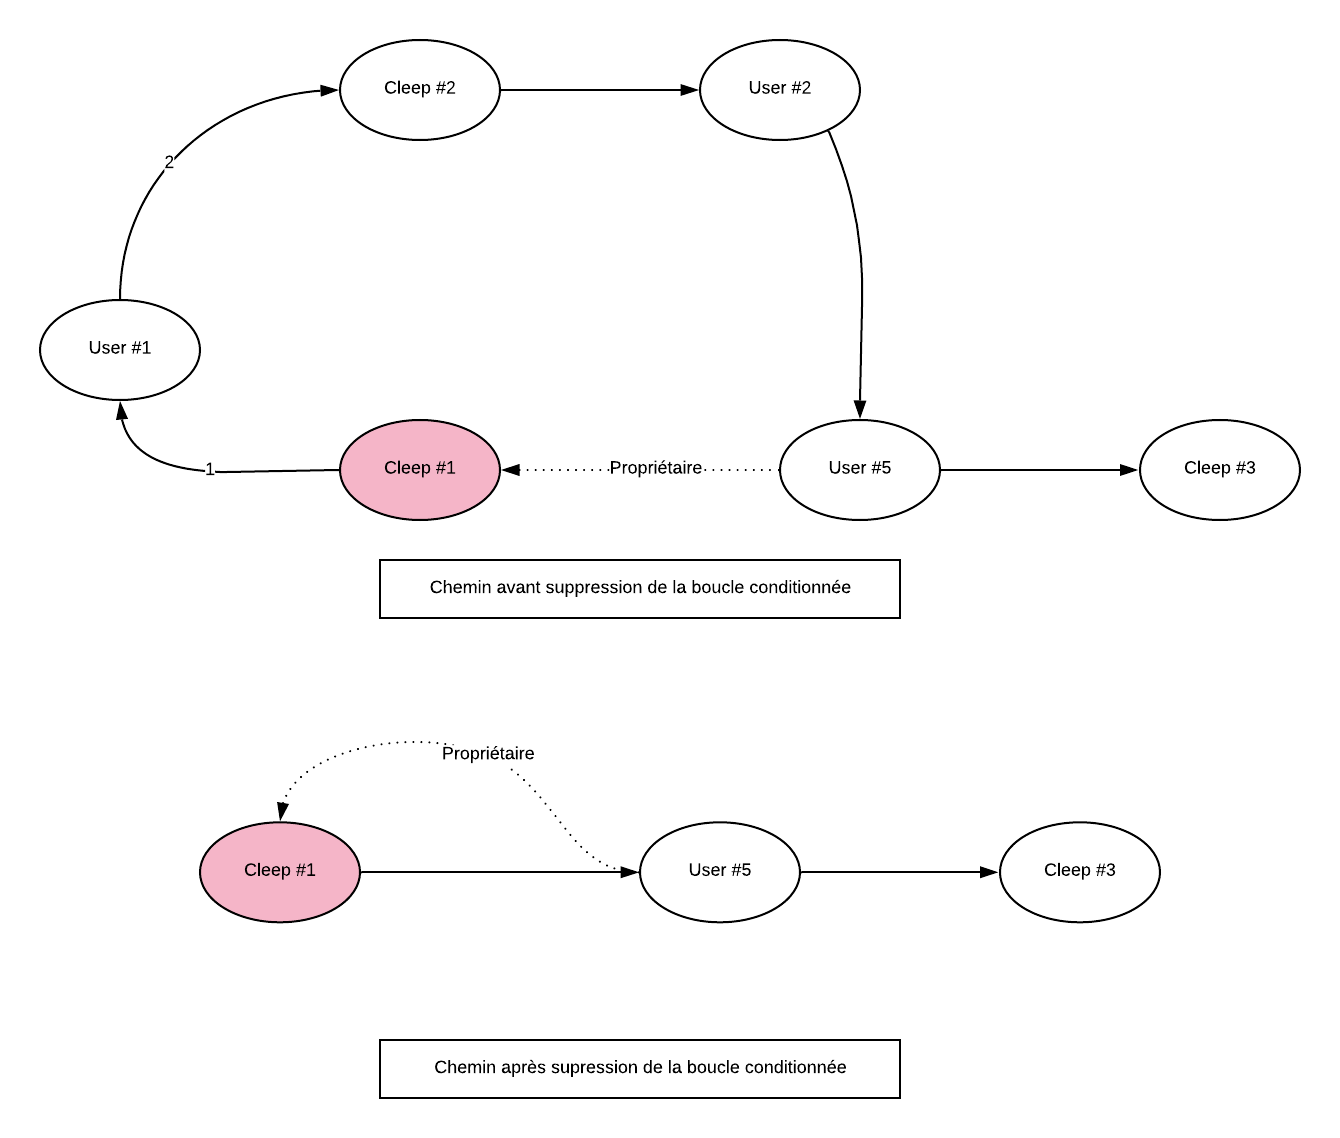
\includegraphics[keepaspectratio = true,scale=0.6]{bbb}
	\caption{Boucle conditionné par la relation cleep $\leftrightarrow$ user}
	\label{fig:bbb}
\end{figure}

La suppression des boucles est une petite optimisation par rapport au reste du travail qui a été fait. Cependant, cela reste dans le but d'avoir des chemins qui avancent en profondeur dans le graphe s'éloignant un maximum du point d'origine. Cela permet aussi d'avoir une certaine uniformité, évitant plusieurs chemins donnant des scores très différents.\\
Ce dernier point est l'une des forces, mais aussi faiblesse de ce moteur de recommandation. C'est la force principale dans le sens où l'utilisation des données intermédiaires permet de comprendre la connexion entre les cleeps. C'est une faiblesse pour les chemins très longs revenant proche du cleep original, l'information sur ce chemin n'est plus assez pertinente par rapport à la proximité.

\newpage

\section{Mission : Aide à l'amélioration d'une plateforme de déploiement pour Sia Partners (2 mois)}
Cette mission est orientée data engineer, développeur backend / frontend et donc est moins orienté dans le traitement et l'analyse de la donnée, mais plus sur l'infrastructure permettant d'utiliser et de présenter au mieux la donnée. Pendant cette mission, la personne référente était Gabriel Creti et Mathieu Thiboust qui ont grandement participé au développement de cette plateforme.
 
\subsection{Présentation du sialab}
La plateforme sialab est composée de deux parties distinctes :
\begin{itemize}
	\item Les bots : l'ensemble des bots developpé par l'équipe datascience en fait partie. Un bot est en général une solution technique developpé par l'équipe datascience de Sia Partners répondant à un problème spécifique. Le bot est utilisable via une interface graphique, le but étant d'avoir un produit fini et pas seulement un algorithme de machine learning. La \textbf{Figure \ref{fig:bot}} est un exemple de bot disponible via la plateforme \cite{bot}.
	\item Les plateformes sialab : Plateformes développées pour les clients. Contrairement aux bots qui sont plus pour un usage démo, les plateformes sialabs sont pour un usage opérationnel. Elles permettent de lancer et programmer des \textbf{tâches}. Les tâches sont des scripts qui ont vocations à être lancer de manière régulières : par exemple, une tâche qui va rechercher des données de manière régulières au travers d'API publiques comme la météo ou le trafic routier. Elles permettent aussi la création de Restful API et d'interfaces personnalisées.
\end{itemize}

\begin{figure}[!h]
	\centering
	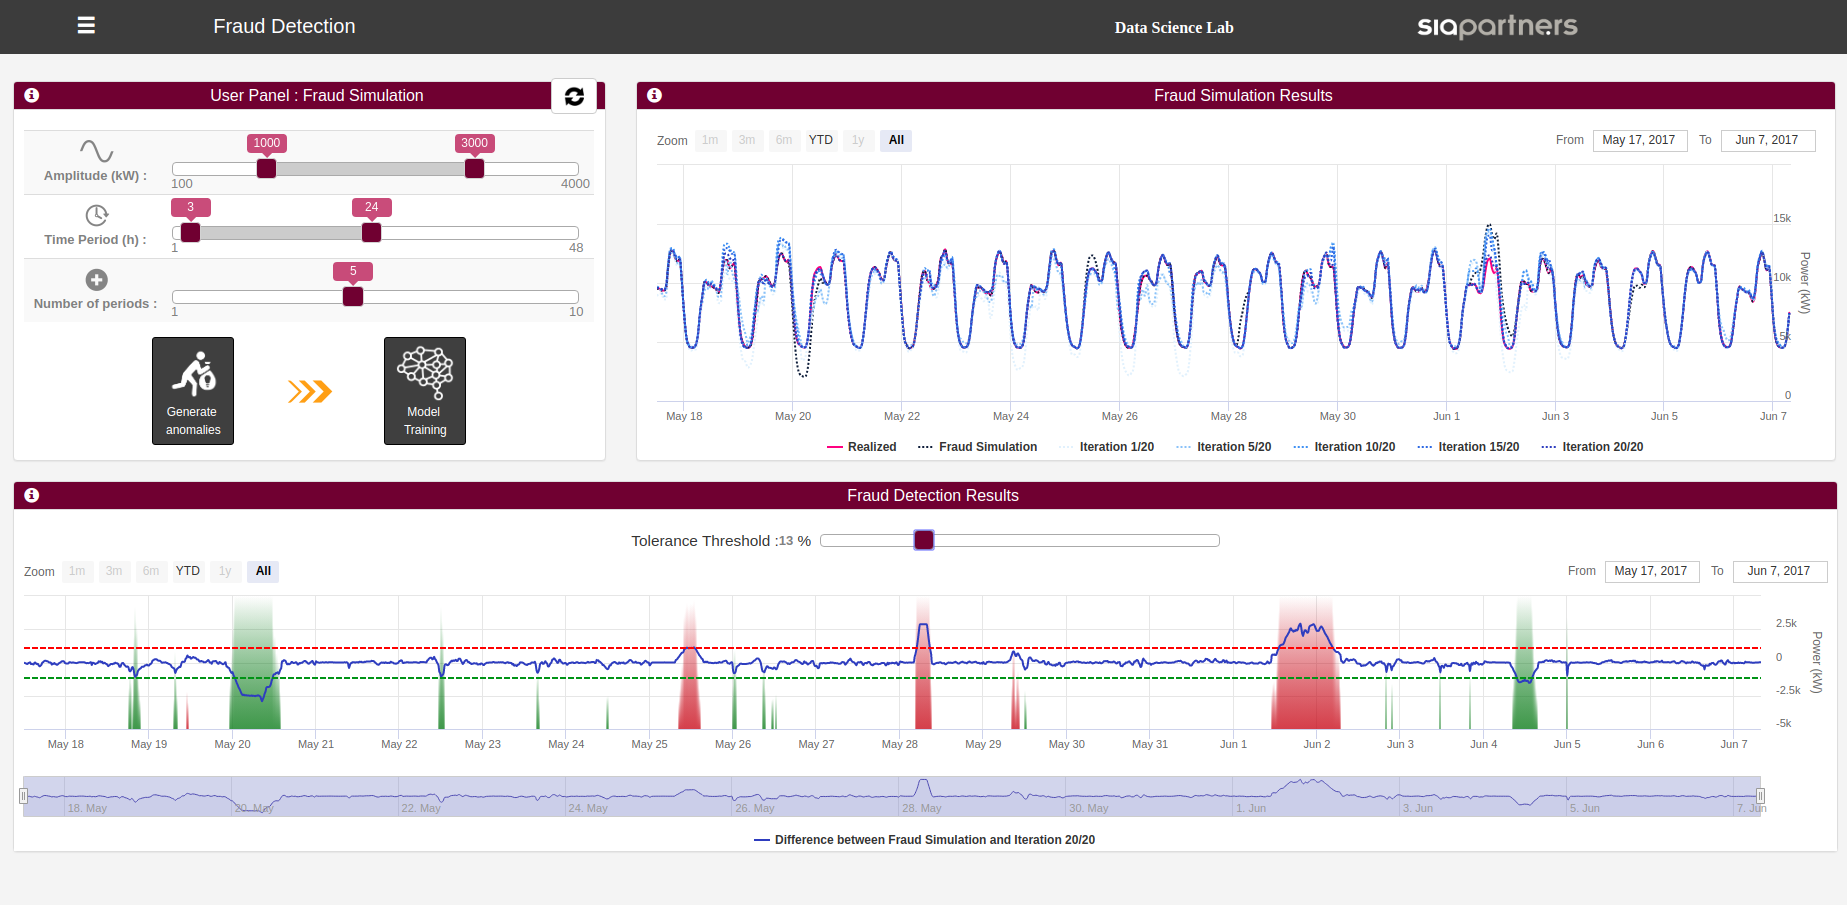
\includegraphics[keepaspectratio = true,scale=0.25]{bot.png}
	\caption{Exemple de bot}
	\label{fig:bot}
\end{figure}

La première version des plateformes sialabs est née d'un besoin client il y a un peu plus de 2 ans. Le client voulait au départ une plateforme mettant à disposition des API à travers lesquels ils pouvaient récupérer ses données de prédiction stockées en base. Ensuite un autre ajout a été très rapidement demandé, celui de pouvoir lancer et programmer des scripts permettant d'avoir ces prédictions. Par la suite, cette plateforme est devenu un argument de vente et plusieurs autres plateformes de ce type ont été créé pour les clients dont un pour Sia Partners permettant de lancer des process internes.\\

Ainsi l'ensemble bots et plateformes est ce que l'on appelle le sialab. 

\subsection{Objectifs et problématique}
Avant mon arrivé, le sialab dans sa première version posait plusieurs problèmes du fait du développement anarchiques des bots et des plateformes.

\subsubsection{Bots\\}
Les développeurs de bots à l'époque étaient obligés de travailler en local, ce qui les obligeaient à installer toutes les librairies qu'ils utilisaient pour ensuite déployer l'application sur un serveur appartenant à Sia Partners ou sur machine virtuel OVH/Amazon etc. Plusieurs problèmes découle alors de ce mode de fonctionnement:

\paragraph{Backups}
Il n'y pas de backups. Les serveurs sur lesquels étaient déployés les bots n'avaient pas de structure permettant de répliquer les applications et avoir un service qui tourne en permanence. Les serveurs étaient donc des points individuels de défaillances (single point of failures). Ainsi les application étaient copiées via une connexion SSH sur les serveurs et accessible via l'adresse : "IP du serveur (ou nom de domaine Sia Partners) " + "nom de l'application". Par exemple : 
\begin{itemize}
	\item Bot KYC Adverse News disponible sur \textit{http://192.95.33.110/shiny/adb1w1b/}.
	\item Bot Reg Review disponible sur \textit{http://regwatch.sia-partners.com/demo}
\end{itemize}


\paragraph{Contrôle de Version}
Les consultants développant en local, et déployant par leurs propres moyens les bots,  utilisaient rarement le logiciel de version de contrôle décentralisé autrement connu sous le nom de git à leur disposition.
Le manque d'utilisation de cet outil entraîne plusieurs autres problèmes qui pour certains projets peuvent faire perdre beaucoup de temps :
\begin{itemize}
	\item Manque de versions fonctionnels du bot (v1, v2 etc)
	\item Pas d'information sur les patchs fait au bots. Donc impossible de restaurer le bot dans un état précédent si la modification ne marche pas sur le serveur.
	\item Pas de backup de code. Donc si le code est perdu sur le serveur et en local, le bot est perdu
\end{itemize}
Cette pratique est très importante, mais du fait des conditions de développements chaotiques, l'habitude n'est pas prise.

\paragraph{La stabilité}
Comme les bots sont éparpillés sur plusieurs serveurs, environ une trentaines différents, chaque serveur avait sa propre configuration. Ainsi pour chaque bot qui venait s'ajouter à un serveur, ajoutait ses dépendances (en terme de librairies mais aussi en termes de services). Il était donc possible de se retrouver avec 2 bots différents sur un serveur, utilisant des librairies qui entrent en conflits.\\
La stabilité n'est donc pas assurée, et les serveurs étaient souvent polluées par plusieurs librairies inutilisées.

\paragraph{L'administration}
Avec autant de serveurs à administrer, il y a autant problèmes possibles, que ce soit en terme de stabilité, d'installation ou tout simplement de problèmes internes aux serveurs (image à mettre à jour etc.).\\
Par ailleurs, il peut y avoir un long moment entre l'apparition d"un bug et la découverte de celui-ci, car aucun serveur n'avait ses logs centralisés. Ainsi, le seul moyen de "trouver" un bug était d'expérimenter le bug ou d'en avoir les retours par les utilisateurs. L'administration devient d'autant plus problématique à chaque ajout de bots. Cette tâche là était donc pénible et faisait perdre beaucoup de temps.

\subsubsection{Plateforme}

\paragraph{Contrôle de Version et Backups}
Comme plusieurs consultants peuvent développer sur la plateforme, le contrôle de version était utilisé. Ainsi le code en lui même de la plateforme était versionné. Ainsi contrairement aux bots, les plateformes possèdaient des backups. De plus la base de donnée reliée avait aussi des backups.\\
Cependant les scripts de déploiement des plateformes n'étaient présents que sur les serveurs et n'étaient pas inclus dans le contrôle de version. Ainsi si un serveur avec une plateforme perdait ses données, le déploiement de cette dernière s'en retrouvait affecté. \\

\paragraph{Stabilité et administration}
Par ailleurs, comme pour les bots, les plateformes étaient aussi éparpillés sur plusieurs serveurs. Ainsi, les même problèmes étaient présents, et la même pénibilité d'administration qui en découle. Cela était d'autant plus problématique que ces plateformes étaient destiné aux clients, donc avec une exigence plus grande concernant la résolution des bugs.

\subsubsection{Objectifs}
Une deuxième version du sialab était en cours de création lorsque j'ai rejoint l'équipe pour participer à son developpement. L'objectif principale de cette mission est de répondre à l'ensemble des problèmes cités précédemment, en particulier avoir une interface d'administration globale permettant d'avoir connaissance rapidement des bugs sur la plateforme.\\

Cela implique aussi de centraliser l'ensemble des projets existants et d'avoir une méthode automatique de déploiement des bots/plateformes. Le but étant de se rapprocher au maximum du déploiement en un clique.\\

Pendant cette mission j'ai travaillé en méthode Agile avec l'équipe sur le projet (Gabriel Creti et Matthieu Thiboust). Chaque semaine il y avait une réunion hebdomadaire avec une liste de tâche à faire et la présentation des avancements qui ont été fait. Cela a permis d'avancer rapidement sur le projet et d'avoir une version stable en Septembre.

\subsection{Travail effectué}
Dans cette section je vais décrire l'ensemble des fonctionnalités nouvelles le travail qui a été fait sur la version 2 du sialab. J'ai participé à toutes les étapes du développement, que ce soit au niveau de l'infrastructure, au niveau du déploiement ou au niveau du développement (frontend et backend) de la plateforme.

\subsubsection{Processus de déploiement}

L'ensemble des problèmes listés auparavant reposaient sur deux éléments:
\begin{itemize}
	\item Le code n'est pas contrôlé : les consultants n'étaient pas "forcés" à utiliser le contrôle de version (git)
	\item Le déploiement n'est pas normalisé : les consultants déployaient leurs bots sur les serveurs qu'ils connaissaient
\end{itemize}
C'est pourquoi l'ensemble de la chaîne de déploiement a été repensé. Cela implique des changement dans la manière de développer mais aussi dans la manière d'utiliser les outils à disposition. 

\subsection{Vision critique et apport personnel}




\newpage


\section{Conclusion}
\newpage

\section{Annexes}
\subsection{Code source allégé du site de la fnac}
%\lstinputlisting[language=html]{fnac.html}
\subsection{Graphe tests ArangoDB / Neo4j}

\begin{figure}[!h]
	\centering
	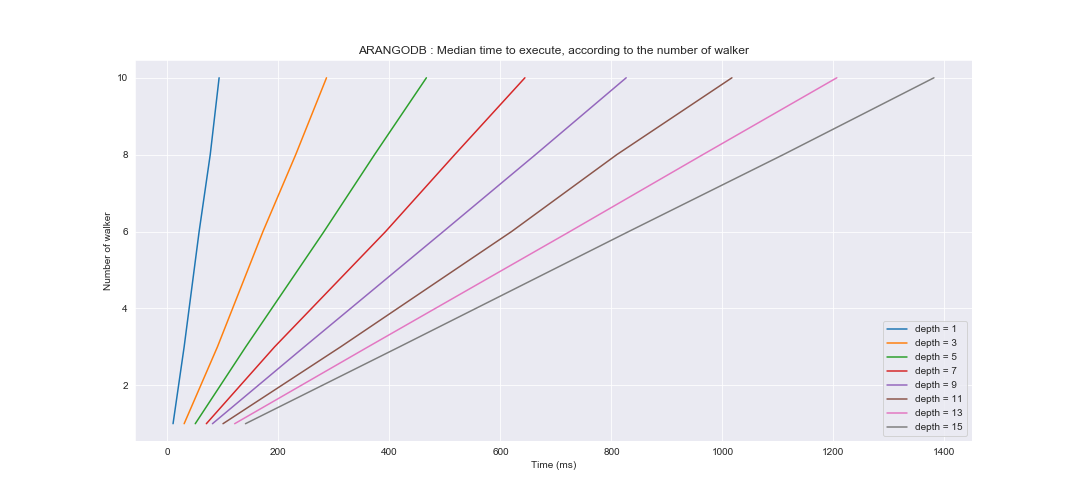
\includegraphics[keepaspectratio = true,scale=0.4]{arangoDB_nbwalker_time.png}
	\caption{Performances d'ArangoDB sur marche aléatoire en fonction du nombre de chemin aléatoire}
	\label{fig:arwalk}
\end{figure}


\begin{figure}[!h]
	\centering
	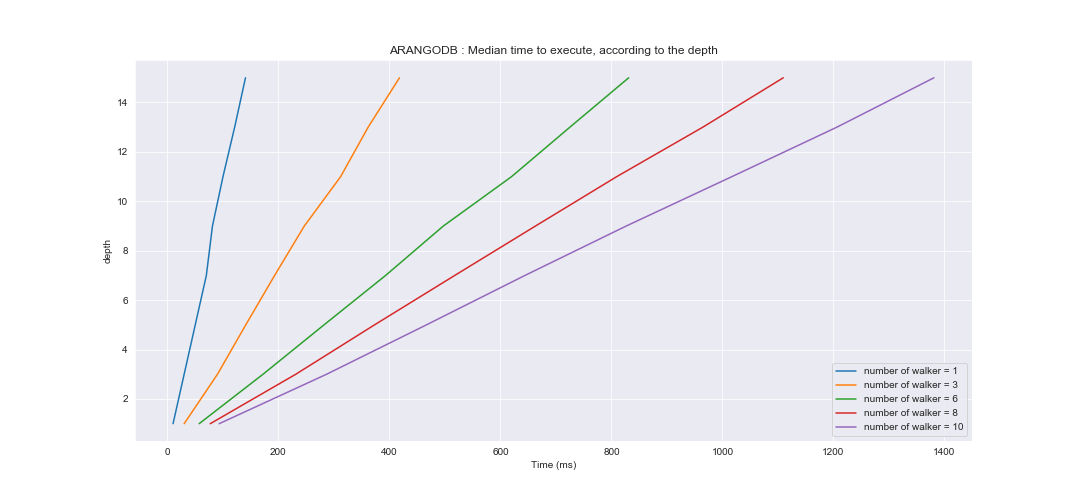
\includegraphics[keepaspectratio = true,scale=0.4]{arangoDB_depth_time.png}
	\caption{Performances d'ArangoDB sur marche aléatoire en fonction de la profondeur}
	\label{fig:ardepth}
\end{figure}
\newpage

\begin{figure}[!h]
	\centering
	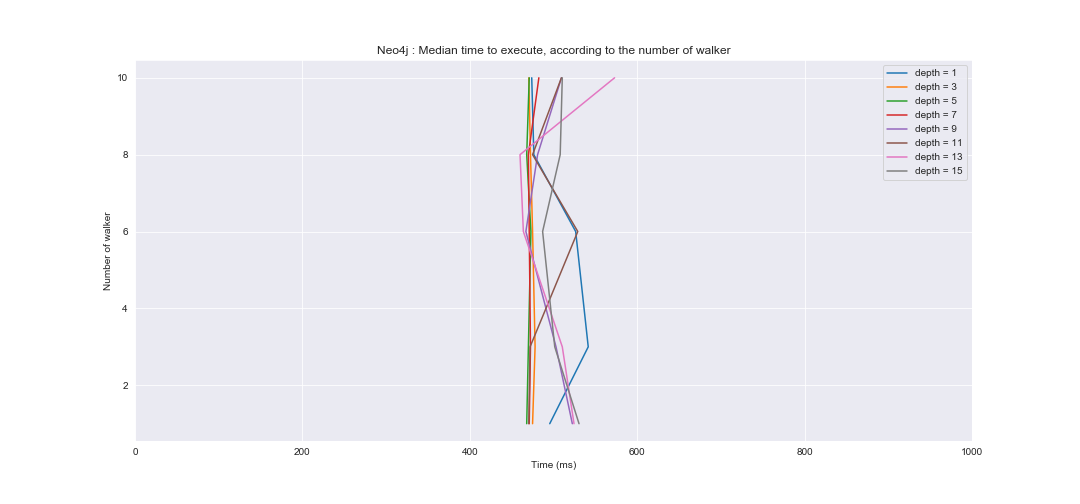
\includegraphics[keepaspectratio = true,scale=0.4]{neo4j_nbwalker_time.png}
	\caption{Performances d'ArangoDB sur marche aléatoire en fonction du nombre de chemin aléatoire}
	\label{fig:newalk}
\end{figure}


\begin{figure}[!h]
	\centering
	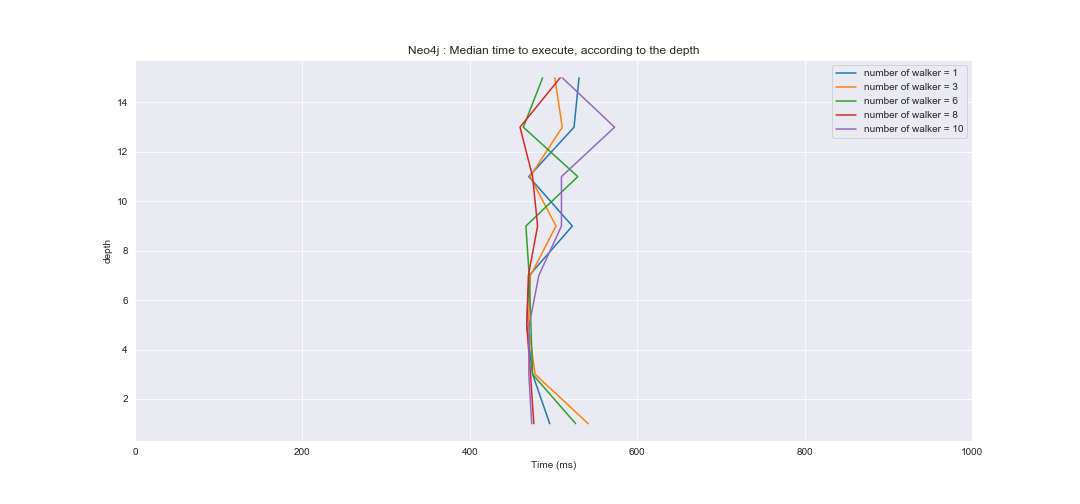
\includegraphics[keepaspectratio = true,scale=0.4]{neo4j_depth_time.png}
	\caption{Performances d'ArangoDB sur marche aléatoire en fonction de la profondeur}
	\label{fig:nedepth}
\end{figure}
\newpage
\subsection{Exemple : Heuristique de Pinterest appliqué au cas de Cleep}

Le graphe \textbf{figure \ref{fig:ex1}} sert d'exemple pour cette partie. Le cleep en rose est le cleep à recommander. Les cleeps violets sont les autres cleeps du graphe et ceux en gris sont les utilisateurs. Pour des raisons de simplicités, je n'ai pas inclus les listes.
\begin{figure}[!h]
	\centering
	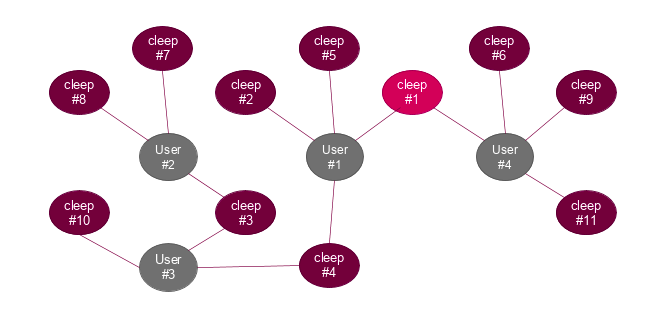
\includegraphics[keepaspectratio = true,scale=0.6]{ex1}
	\caption{Graphe de départ}
	\label{fig:ex1}
\end{figure}

Les \textbf{figures \ref{fig:ex2}, \ref{fig:ex3}, \ref{fig:ex4}} décrivent le processus de chemin aléatoire. Dans cet exemple, il y a 3 marches aléatoire effectuées (désignées par les chemins vert) donc 3 cleeps possiblement recommandés : les cleeps \#8, \#10 et \#11.
\begin{figure}[!h]
	\centering
	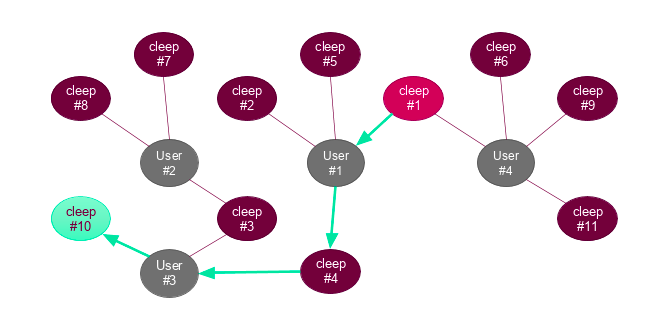
\includegraphics[keepaspectratio = true,scale=0.6]{ex2}
	\caption{Chemin aléatoire n°1}
	\label{fig:ex2}
\end{figure}

\begin{figure}[!h]
	\centering
	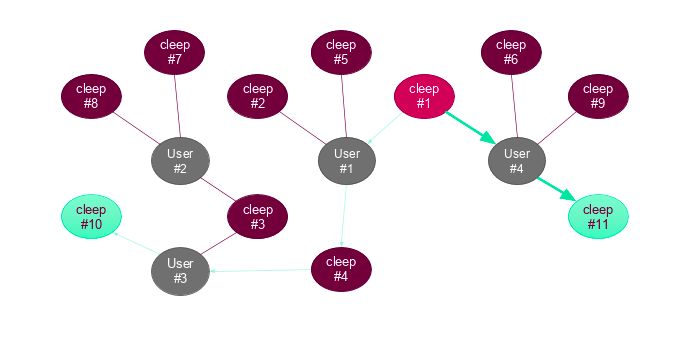
\includegraphics[keepaspectratio = true,scale=0.6]{ex3}
	\caption{Chemin aléatoire n°2}
	\label{fig:ex3}
\end{figure}

\begin{figure}[!h]
	\centering
	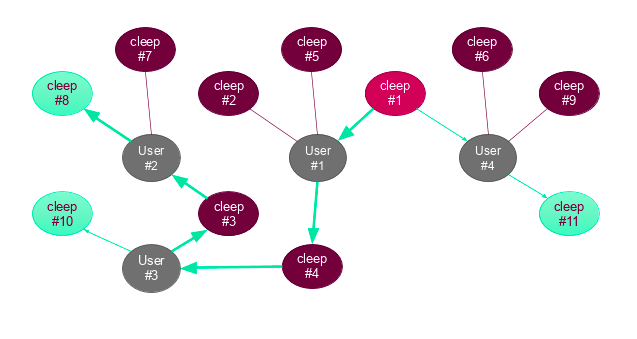
\includegraphics[keepaspectratio = true,scale=0.6]{ex4}
	\caption{Chemin aléatoire n°3}
	\label{fig:ex4}
\end{figure}

La \textbf{figure \ref{fig:ex5}} décrit le processus de selection des meilleurs cleeps. Les cleeps se voient d'abord appliquer un score. Si ce score dépasse un certain seuil comme c'est le cas pour les cleeps \#10 et \#11, alors ces cleeps peuvent être poussés comme recommandations.

\begin{figure}[!h]
	\centering
	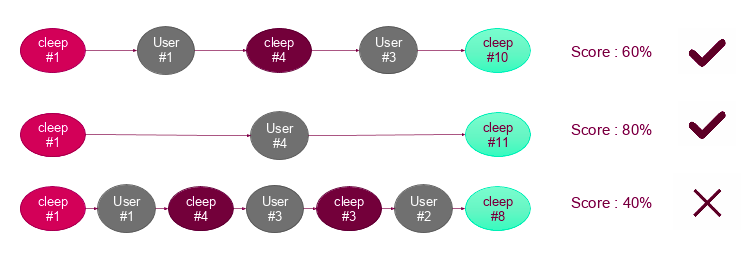
\includegraphics[keepaspectratio = true,scale=0.6]{ex5}
	\caption{}
	\label{fig:ex5}
\end{figure}


\newpage

\section{Glossaire}
\begin{thebibliography}{9}
	\bibitem{cleep} 
	Site de Cleep : \textit{https://app.cleep.io/}
	\bibitem{fnac} 
	Exemple de la Fnac : \textit{https://livre.fnac.com/a13195869/Agnes-Martin-Lugand-A-la-lumiere-du-petit-matin}
	\bibitem{mve}
	Exemple site internet avec plusieurs produits : \textit{https://livre.fnac.com}
	\bibitem{levenshtein}
	Approfondissement sur la \\
	 de Levenshtein : \textit{https://en.wikipedia.org/wiki/Levenshtein\_distance}
	\bibitem{pixie}
	Pixie: A System for Recommending 3+ Billion Items to 200+ Million Users in Real-Time :
	\textit{https://labs.pinterest.com/user/themes/pin\_labs/assets/paper/paper-pixie.pdf}\\
	Auteurs : Chantat Eksombatchai, Pranav Jindal, Jerry Zitao Liu, Yuchen Liu,
	Rahul Sharma, Charles Sugnet, Mark Ulrich, Jure Leskovec
	\bibitem{Pinterest}
	Site Internet de Pinterest: \textit{https://www.pinterest.com/}
	\bibitem{neo4j}
	Documentation sur les algorithmes de neo4j: \\ \textit{https://neo4j.com/docs/graph-algorithms/current/experimental-algorithms/}
	\bibitem{cypher}
	Documentation sur Cypher :\\
	\textit{https://neo4j.com/docs/cypher-manual/current/introduction/\#cypher-introduction}
	\bibitem{aggrg}
	Fonction d'aggregation sur Cypher:\\
	\textit{https://neo4j.com/docs/java-reference/current/extending-neo4j/procedures-and-functions/aggregation-functions/}
	\bibitem{bot}
	Bot détection de fraude:\\
	\textit{https://lab.sia-partners.ai/showroom/fraud-detection/}
	
\end{thebibliography}
\newpage






% back cover
\imtaMakeCover

\end{document}
%%%%%%%%%% END %%%%%%%%%% 
%%%%%%%%%%%%%%%%%%%%%%%%% 
